\pagestyle{plain}
\chapter{Introdução}

As ações de consumo humano agridem a natureza em quase todos os processos, muitas vezes o processo é irrefreável, os riscos e danos são previstos, demostrando a necessidade e importância de existir uma política corporativa que preze pela sustentabilidade \cite{Melo2020}. Esta sustentabilidade tem o compromisso de explorar a natureza de forma cíclica, interferindo o mínimo possível no meio, ela exige respeito ao meio ambiente, em situações como a atividade industrial, percebe-se que se retira da natureza sua matéria-prima e recursos energéticos, os quais são escassos e limitados e necessitam de reposição para se manter cíclico e sustentável temporalmente \cite{DeSouza2019}. A sustentabilidade é vista neste sentido como uma forma de minimizar o impacto humano na natureza e preservar os recursos naturais para as gerações futuras. Ela envolve um compromisso com o respeito a esse conjunto de elementos biológicos, evitando a extração excessiva de recursos naturais e a poluição do ar, água e solo.

Uma possibilidade de concretude empresarial sobre a sustentabilidade é a implementação de uma gestão ativa de marca. A exemplo \cite{Gupta2013SustainabilityPerformance} Apresentam um arcabouço conceitual fundamentado na teoria do triple bottom line com base no pressuposto de que a marca como fator estimulante pode acelerar a conversão das oportunidades disponíveis para um negócio em desempenho superior, tanto para ganhos financeiros quanto para sustentabilidade ambiental. Neste sentido esta pesquisa visa formular um modelo empírico para validação de marcas baseadas nos elementos relacionados à sustentabilidade ambiental da Amazônia do Brasil.


\section{Tema e Problema}
\subsection{Problema do estudo}

Relações percebidas por consumidores sobre a sustentabilidade ambiental da Amazônia e marcas locais potencializam a confiabilidade e a predileção aos produtos desenvolvidos, capazes de compor um modelo empírico de \textit{Branding}, tendo como base o \textit{Brand Equity} sustentável.

\subsection{Questões de pesquisa}

- Preferências relacionadas à conexão dos consumidores quanto à marca podem ser acionadas quando empresas usam conceitos ligados à sustentabilidade ambiental como estratégia de \textit{Branding}?

- Estruturas particulares, processos de interação e configurações gráficas em produtos com \textit{Branding} voltado a produtos de empresas sustentáveis facilitam a percepção do consumidor no que tange ao conceito de responsabilidade social e ambiental da empresa?

- Conceitos relacionados à sustentabilidade ambiental como pressuposto de confiança posicionam estrategicamente a empresa numa fidelidade à marca.

- Marcas das empresas associadas à sustentabilidade ambiental da Amazônia contêm ativos sociais autênticos hábeis a formar nos consumidores um conhecimento da marca positivo?

- Marcas usando estratégias sustentáveis podem desenvolver um valor adicional na área de responsabilidade ambiental em detrimento das que não usam.

\subsection{Hipóteses}

\begin{itemize}
    \item  A percepção de consumidores e gestores sobre marcas que utilizam a sustentabilidade ambiental como \textit{brand equity} influencia positivamente a fidelidade dos consumidores.
    \item Informações geradas pela  percepção de consumidores e gestores sobre marcas que utilizam a sustentabilidade ambiental como \textit{brand equity} possibilitam desenvolver  um modelo empírico de Branding.
\end{itemize}


\section{Objetivos}
\subsection{Objetivos gerais}

Formular e validar um modelo empírico para validação de marcas baseadas nos elementos relacionados à sustentabilidade ambiental da Amazônia do Brasil.

\subsection{Objetivos específicos}

 
    - Analisar estudos sobre \textit{Branding} e marcas sustentáveis, bem como detalhar os avanços do empreendedorismo ambiental para o ecossistema florestal com atividade extensiva;
    
    - Testar as propriedades psicométricas de precisão e validade de uma escala para avaliação do valor da marca com base na sustentabilidade ambiental;
    
    - Investigar e analisar os construtos do \textit{brand equity} baseado em marcas relacionadas à sustentabilidade ambiental da Amazônia que influenciam a fidelidade do consumidor e a intenção de compra de seus produtos;
    
    - Determinar quais os elementos a partir da percepção dos empreendedores de marcas relacionadas à sustentabilidade ambiental da Amazônia do Brasil influenciam para autenticidade da marca e como pode influenciar na confiabilidade do consumidor e a subsequente preferência pelo produto vinculado a esta empresa;
    
    - Apresentar um modelo de \textit{Branding} que abranja a gestão estratégica da identidade, posicionamento e comunicação de marcas sustentáveis da floresta amazônica do Brasil, a partir de dados empíricos.
    

%- Propor um serious games do tipo cards para o desenvolvimento de novas marcas sustentáveis.


\section{Justificativa}

Para mitigar tais danos ao meio ambiente sem impactar financeiramente o negócio, diversas empresas, principalmente as que dependem diretamente dos recursos naturais florestais, têm buscado criar e implementar políticas de Responsabilidade Social Corporativa (RSC) baseadas na sustentabilidade ambiental \cite{Orlitzky2011StrategicSustainability}. Tais políticas estão vinculadas diretamente a atividades que usufruem das paisagens naturais sem agressão ao meio ambiente e que, por meio da promoção midiática de sua imagem, aumentam a competitividade e a reputação de uma empresa \cite{Trendafilova2013CorporateField}. Porém, a implantação de políticas baseadas na RSC depende de recursos que invariavelmente modificam os meios de produção e negociação, impactando significativamente o custo final do produto e o lucro a ser obtido. Buscando mitigar tais divergências, empresas investem em construção de marcas focadas na obtenção de clientes que se relacionam diretamente com a sustentabilidade ambiental \cite{Kumar2014SustainabilityPerspective}.

Antes que uma empresa possa impulsionar um negócio com modificações e novos preços para produtos ou serviços, ela precisa considerar sua estratégia de marca \cite{Foroudi20201}. Tais empresas devem considerar como ponto de partida suas relações e atitudes que impactam na percepção dos consumidores frente a  sua marca. Especificamente, isso significa considerar as percepções dos clientes sobre o \textit{Branding} empresarial e esforços relacionados ao tratamento dos valores éticos e morais dos consumidores \cite{Figueiredo2019PassengersBrazil}. Para isso, setores de marketing e \textit{Branding} têm trabalhado diretamente nas imagens mentais desenvolvidas por empresas incluídas no \textit{Brand Equity} de suas marcas, capazes de influenciar consumidores e aumentando as atitudes e a vontade de comprar seus produtos \cite{Schlosser2003ExperiencingIntentions}. 


As marcas gradualmente se tornaram a dimensão central e o ativo estratégico mais importante do marketing de organizações em todas as suas dimensões e muitas empresas adotam várias formas de atividades de marketing verde como parte das suas estratégias \cite{Peattie2005GreenProphesy,Premi202139}. Atividades de tomada de decisão sobre \textit{Branding} que usam novos métodos frequentemente envolvem extensa pesquisa em uma abundante de literatura. Tais atividades são trabalhosas, demoradas e difíceis de ser interpretadas pelos pesquisadores e muito restritas aos conhecimentos empíricos dos empreendedores, que adquirem, ao longo do tempo de trabalho, a partir de erros e acertos \cite{Santos2022BrandFlorestal}. Buscando compreender as dimensões que compõem as nuances do empreendedorismo, se faz necessário estabelecer um cenário atual do desenvolvimento de tecnologias gerenciais, mais precisamente as relacionadas ao marketing de marcas, direcionadas à sustentabilidade ambiental, de maneira que, decisões mais estratégicas sejam tomadas, buscando o engajamento de novos empreendedores à sustentabilidade ambiental efetiva \cite{Mahmood2022TheMatter}. A aquisição destes conhecimentos impacta significativamente em todas as áreas do negócio, influenciando diretamente na capacidade competitiva \cite{Kitchenham2004}. 

Para as pequenas empresas que não possuem capacidade de investimento em Pesquisa e Desenvolvimento (P \&D), observa-se uma redução da competitividade ao longo dos anos, muito por conta do comportamento do consumidor e de suas necessidades \cite{Yenipazarli2019IncentivesTaxation}. Quando observadas marcas que já aplicam políticas sustentáveis em seus empreendimentos, parece vantajoso ter conhecimento, a partir de afirmações encontradas especialmente nos conhecimentos empíricos organizados e assertivos pertencentes aos empreendedores já consolidados, sobre atividades de tomada de decisão a partir do \textit{Branding} e, a partir destas informações, fornecer a novos empreendedores informações que otimizarão o tempo e o trabalho.

Neste sentido, uma pesquisa que analise e desenvolva um modelo efetivo que oriente o desenvolvimento de um \textit{Branding}, a partir dos conhecimentos e opiniões de empreendedores que já desenvolvem seus negócios, tomando como base a responsabilidade social corporativa, apontará os principais indicadores que levam uma marca ao posicionamento estratégico e, por conseguinte, um efetivo alcance de venda. Estes dados podem também fomentar desenvolvimentos científicos e tecnológicos futuros capazes de intervir positivamente no campo, visto que anteciparia a predileção dos consumidores por produtos oriundos da sustentabilidade ambiental, possibilitando, desta forma, o desenvolvimento de empresas mais focadas na sustentabilidade ambiental, e uma produção com menos impacto no meio florestal.

\section{Delineamento do estudo}

Este estudo se apresenta como um trabalho de pesquisa exploratória quantitativa de conteúdos, bem como de estudo de caso. A metodologia utilizada para o desenvolvimento contará com a estruturada em quatro fases:

\begin{enumerate}[label=\bfseries(\Roman*)] 
  - Revisão sistemática dos conteúdos bibliográficos e documentais;
  - Desenvolvimento do Instrumento de coleta de dados e ferramenta psicométrica, como compreender quais os componentes da experiência do usuário são envolvidos na percepção dos consumidores ao visualizar uma marca ligada à sustentabilidade ambiental;
  - Interpretação dos construtos formadores do \textit{Brand loyalty} e qualidade percebida;
  - Avaliação da percepção dos empreendedores por \textit{Grounded Theory};
  - Desenvolvimento do Modelo conceitual para validação de marcas empresariais vinculadas à sustentabilidade ambiental, tendo como base a experiência do usuário relacionada à percepção da marca;
\end{enumerate}

\section{Procedimentos metodológicos}
%%%%CAPÍTULO 1
\subsection{Revisão de escopo: Protocolo adotado}

Buscando contemplar o desenvolvimento das fases deste estudo, dois revisores examinaram independentemente os resultados dos dados obtidos em cada umas das rodadas desta pesquisa. Para isto, foram adaptadas as recomendações do \textit{Cochrane Handbook for Systematic Reviews of Interventions} \cite{Higgins2020}, adotando como procedimentos deste estudo as sete rodadas: (i) Formulação da pergunta, (ii) Localização dos estudos (artigos), (iii) Seleção dos estudos, (iv) Extração dos estudos, (v) Análise e interpretação dos dados e (vi) Síntese da revisão e (vii) qualificação dos trabalhos. Para isto, como modelo estrutural, este trabalho adotou como diretriz o método sistemático \textit{Cochrane Central Register of Controlled Trials} \cite{Bell2005}, adaptando-o para esta pesquisa. 

\subsubsection*{Leis norteadoras da Revisão Sistemática}

As análises sistemáticas de dados bibliométricos e de conteúdos direcionadas para investigações acadêmico-científicas buscam mapear um determinado campo do conhecimento, considerando, em sua maioria, dados textuais de similitude, análises de formação de redes de cocitação, coautoria e relação pesquisa e conteúdo. Buscando tais análises desenvolvidas três principais leis de investigações de caráter bibliométricas, (i) lei da produtividade de pesquisadores conhecida como a lei de \citeonline{Lotka1926}; (ii) lei de dispersão do conhecimento científico ou lei de Bradford; e (iii) lei da distribuição e frequência de palavras em um texto ou lei de Zipf.

A lei da produtividade de pesquisadores consiste no estudo sobre a produtividade acadêmico-científica, baseando-se na proporção produzida pelo meio acadêmico, tendo como base o número de autores sobre determinado campo de estudo científica, mediante ao número de autores \cite{Lotka1926}. Segundo essa lei, o número de autores que realizam “n” contribuições em um determinado campo científico é de cerca de 1/n² daqueles que efetuam uma só, além de que a proporção daqueles que realizam uma única contribuição é de cerca de 60\% \cite{Candido2018}, fundamenta-se no fato de que, supostamente, os pesquisadores com maior prestígio, considerados especialistas na área produzem muito a respeito de um determinado assunto, enquanto muitos pesquisadores produzem uma menor quantidade sobre o mesmo assunto \cite{Hassan2014}.

A lei de dispersão do conhecimento científico tem como base o resultado da produtividade dos periódicos, buscando estabelecer núcleos sobre determinados assuntos específicos. Ela baseia-se na explicação de eventos probabilísticos que se juntam para criar o padrão regular de dispersão de artigos em vários periódicos. O estudo deste fenômeno, por meio da lei de \citeonline{Bradford1934}, possibilita a estimação do grau de relevância de um periódico, já que ela permite, com a mensuração da produtividade dos periódicos, indicar o núcleo e as áreas dispersas relativos a um assunto no mesmo conjunto de periódicos \cite{Sembay2020}. A especialização em determinado tema por um periódico confere a este, qualidade, relevância e maior impacto científico. Já os que apresentam dispersão, demonstram menor relevância para a área temática de estudo \cite{Silva2018}.

A lei de Zipf (lei de frequência e distribuição de palavras em um texto) analisa a ocorrência de palavras em vários documentos apresentando escalonadamente os termos de determinado assunto, o que permite mostrar correlações entre as diferentes palavras e a frequência de seus usos. Ela está balizada no pressuposto que em um texto com um número grande de palavras, a frequência \textit{f} de ocorrência de uma palavra como uma função da posição r deste evento em uma lista ordenada pela frequência de ocorrência é dada por uma lei de potências \cite{Saichev2009,Santos2009}. 

Por meio desta lei associada ao  método de análise de conteúdo é possível determinar estatisticamente a frequência, associação e comportamento do uso dos termos observados \cite{Mozzato2011}, já que o método de análise do conteúdo trata-se de um conjunto de técnicas aplicadas para a análise de dados qualitativos, que se utilizam da ocorrência de palavras e similitudes dos termos concentrados em corpus textuais, tais como resultados, discussão \textit{abstract} e palavras-chave, de modo a determinar a importância destas no contexto do assunto abordado \cite{Cassettari2015}. A Análise de Conteúdo aparece como uma das metodologias mais frequentemente utilizadas nos estudos publicados em periódicos de relevância quando se compreenderá o comportamento de corpus textuais extensos \cite{Lima2021}, demostrando ser um método de relevância de estudos exploratórios, tais como revisões sistemáticas \cite{Klant2021}.

A conjunção destas leis e métodos analíticos associáveis de modo a explanar determinado conteúdo, apresenta constatações relevantes para uma melhor compreensão dos estudos quantitativos. Após essas abordagens-base desta revisão de metadados, foi possível constar lacunas na literatura dos campos do conhecimento científico sobre a sustentabilidade ambiental e relação com negócios e marcas.

\subsubsection*{Delineamento Procedimental da Revisão Sistemática}


\subsubsection*{Extração dos estudos}

A partir dos bancos de dados disponíveis pelo acesso periódico capes, foi Inicialmente realizada uma busca com descritores primários nas bases de dados Scopus (Elsevier) e \textit{Web of Science} (Clarivate Analytics). Como estratégia para busca da produção acadêmica a ser utilizada nesta rotina, foram definidos descritores primários utilizando a lógica baseada em termos centrais. Os descritores foram trabalhados na língua inglesa, vinculados por operadores booleanos (AND, OR e NOT), seguindo as regras descritas por \citeonline{Slamet2016} e vinculados ao tema proposto para artigos publicados entre 2016 e 2022. O critério de inclusão e exclusão para esta rodada das recomendações aceitou apenas artigos completos, escritos na língua inglesa e apresentam os descritores primários nos seguintes campos: título (title), resumo (abstract) e palavras-chave (keywords).

\subsubsection*{Rodada 1: Seleção dos dados}

\subsubsection*{\textit{Seleção automática}}

Haja vista a possibilidade de se trabalhar com dois bancos de dados, a seleção inicial dos estudos foi realizada na sua primeira fase utilizando a “Busca por trabalhos duplicados”, a partir da seleção dos artigos únicos com o emprego do software Start (\textit{State of the Art through Systematic Review}). O sistema Stat adota como principal classificador automático o método (SCAS) seleção automática de citação de pontuação. O SCAS classifica os artigos utilizando duas fases, a primeira é dividida em dois recursos: por pontuação e por citação, já a segunda fase classifica em quadrantes \cite{Octaviano2015}.

Na primeira fase, o SCAS adota uma classificação de escore por valor em que, para cada ocorrência dos descritores contidos nos campos: título, resumo e palavras-chave, ele confere um determinado valor previamente atribuído. Nesta pesquisa, foram consideradas as pontuações de 5 pontos no título, 3 pontos no resumo e 2 pontos nas palavras-chave, os descritores adotados nesta fase foram: \textit{Agriculture, Entrepreneurship, Extensionist, Farming} e \textit{Tith}.
Já na segunda fase do SCAS, o método posiciona os artigos em duas categorias que contêm quatro quadrantes hierarquicamente determinados pela Hipp (Hierarchical Point Placement). \citeonline{Paulovich2008} descrevem as categorias da seguinte forma:

\begin{enumerate}
  - Categoria 1. São analisados e classificados automaticamente nesta categoria os artigos categorizados nos quadrantes Q1 e Q4, onde o quadrante Q1 inclui automaticamente todos os artigos já analisados e aceitos e o quadrante Q4 exclui automaticamente todos os artigos já analisados e excluídos;
  
   - Categoria 2. São analisados e classificados automaticamente nesta categoria os artigos categorizados nos quadrantes Q2 e Q3, onde o quadrante Q2 inclui automaticamente artigos a serem aceitos manualmente pelo avaliador, já para o Q3, o sistema inclui os artigos rejeitados por pontuação baixa mais passiveis de inclusão no Q2 e posterior seleção manual pelo avaliador.
\end{enumerate}

Na Figura \ref{fig:1} é possível compreender os quatro quadrantes adotados neste método.

\begin{figure}[H]
  \centering
  \caption{Quadrantes e categorias adotadas no posicionamento hierárquico de pontos}
  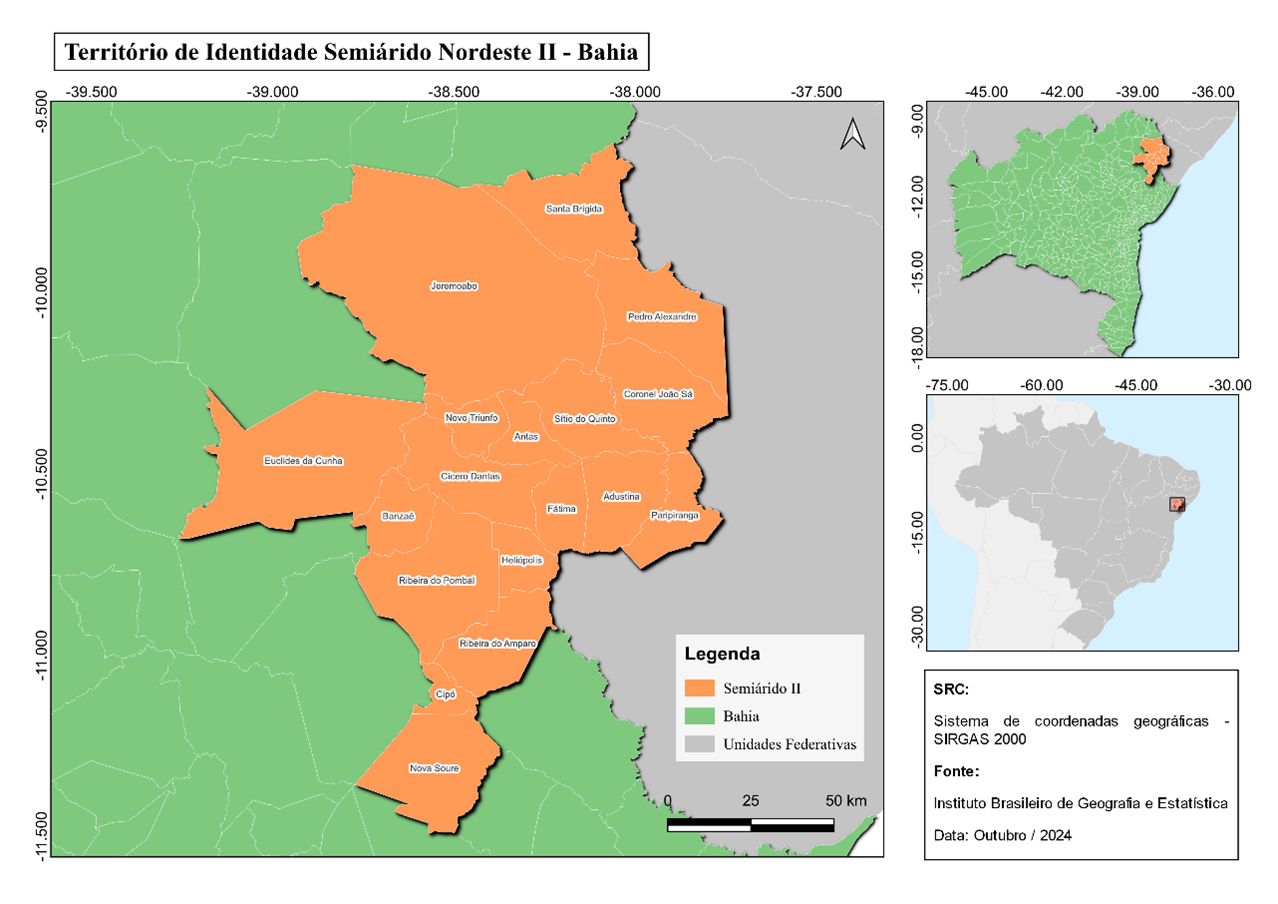
\includegraphics[scale=0.5]{Imagens/fig_1.pdf}
  \fonte{\textbf{Elaborado pelos autores} (2022)}
  \label{fig:1}
\end{figure}

De modo a completar a extração dos artigos classificados no Q2, os artigos classificados neste quadrante, foram lidos títulos, resumos, e palavras-chave para verificação efetiva da inclusão ou exclusão.

\subsubsection*{\textit{Seleção manual}}

Buscando mitigar possíveis artigos não relacionados ao tema proposto, foram selecionados os artigos que apresentaram valores maiores nos índices de inclusão descritos na Tabela \ref{tab:1} para poder ser elegível à próxima rodada.


\begin{table}[H]
  \centering
  \caption{Critérios de Inclusão/Exclusão dos artigos observados}
  \label{tab:1}
  \resizebox{\columnwidth}{!}{%
    \begin{tabular}{lc}
      \hline
      \multicolumn{1}{c}{\textbf{Critérios}}                     & \textbf{Grupo de índices}  \\ \hline
      Apresenta os dois descritores no título                  & Inclusão (I)               \\
      Periódico com Alto Fator de impacto             & Inclusão (I)               \\
    Correlação   entre as duas áreas temáticas                 & Inclusão (I)               \\
      Não é   trabalho sobre temas relacionados                  & Exclusão (E)               \\
      Não é   trabalho sobre métodos inovadores                  & Exclusão (E)               \\
      Não   apresenta solução inovadora                          & Exclusão (E)               \\
      Não   apresenta possibilidade de replicação do experimento & Exclusão (E)               \\
      É uma   revisão bibliográfica                              & Exclusão (E)               \\
      Pouca   aderência aos descritores primários                & Exclusão (E)               \\ \hline
    \end{tabular}%
  }
\end{table}

Os demais trabalhos são considerados automaticamente inelegíveis para a próxima rodada. Todas as seleções nesta rodada foram realizadas por dois pesquisadores, independentemente e restrita de modo a evitar influência pessoal nos resultados, as discrepâncias observadas durante esta rodada foram resolvidas por consenso.

\subsubsection*{Rodada 2: Extração dos dados}

\subsubsection*{\textit{Dados categóricos nominais}}
 Para classificação de qualidade dos artigos selecionados, foram adotados três classificadores, atribuído 1 ponto para cada classificador obtido:
 
\begin{enumerate}[label=(\alph*)]
- Fator de impacto segundo Qualis capes 2016 para a área de avaliação Ciências Agrárias I, pois o CAPES classifica os extratos utilizando bases indexadoras tais como o JCR (Journal Citation Report) ou Scimago (2 years/doc). Cada extrato possui uma pontuação que varia de 0 a 100, quando considerados termos palavras se classifica o Qualis utilizando o JCR, podemos observar os valores de classificação como sendo: A1 - JCR ranking > 75\%, A2 - JCR ranking entre 55 e 75 \%, A3 - JCR ranking entre 35 e 55 \%, A4 - JCR ranking entre 15 e 35 \%,  B1 -SCOPUS ranking > 50 \%,  se não está no JCR ou se está no JCR < 15 \%, B2 -SCOPUS ranking entre 40 e 50 \%, se não está no JCR, B3 - SCOPUS ranking entre 25 e 40 \% se não está no JCR e B4 - SCOPUS ranking < 25 \% se não está no JCR.
- Classificação do modelo econômico agrícola (Agricultura sustentável, Agricultura Campesina, Associação ou Cooperativismo, agricultura extensiva) e sistema de produção (Agricultura ou Pecuária);
- E categoria de empreendedor, segundo a definição de \citeonline{Zuini2014} (Empreendedor Informal, empreendedor cooperado, empreendedor agrícola digital, empreendedor feminino, empreendedor individual, empreendedor social).
\end{enumerate}

A seleção ocorrerá manualmente, sendo possível, assim, realizar uma leitura mais aprofundada, buscando a compreensão de todo o conteúdo desenvolvido nos manuscritos, assim como a relação de causa/efeito das atitudes empreendedoras relacionadas à produção agrícola sustentável. 

Para valores dos dados categóricos, foram atribuídos os valores de 0 não atendem o indicador, 0.5 atende parcialmente o indicador e 1 atende o indicador, assim como os valores alcançados no ranking de prioridade (3 Muito alto, 2 Alto e 1 Baixo).

Nesta fase, foram excluídos os manuscritos que apresentavam relativas similaridades com os demais, assim como trabalhos que mantinham caráter de continuidade de uma pesquisa macro, pelos mesmos autores ou grupo de pesquisa.

\subsubsection*{\textit{Dados categóricos ordinais}}

Buscando atender aos critérios de qualidade dos trabalhos selecionados, nesta fase de síntese, foram desenvolvidos códigos de indicadores de qualidade (Tabela \ref{tab:2}), adotados para a classificação por índice, o modelo de escala Likert partido do valor mais baixo 0 (Não atende o indicador) para o valor mais alto 5 (Atende completamente o indicador). Os artigos que pontuaram com > 21 foram considerados muito alto, entre 21 e 13,  foram considerados alto, e artigos que alcançaram pontuação de < 13 foram considerados baixos, nesta rodada não foram excluídos artigos.



\begin{table}[H]
  \centering
  \caption{Indicadores adotados para descrição de qualidade dos artigos.}
  \label{tab:2}
  \resizebox{\textwidth}{!}{%
    \begin{tabular}{lll}
      \hline
      \multicolumn{1}{c}{\textbf{Siglas}} & \multicolumn{1}{c}{\textbf{Indicador}}                             & \multicolumn{1}{c}{\textbf{Grupo de Índice}} \\ \hline
      DME                                 & Descreve   o método e os meios econômicos adotados                      & Índices de qualidade                         \\
      TEA                                 & Apresenta   o tipo de negócio adotado                     & Índices de qualidade                         \\
      ACR                                 & Apresenta   capacidade de reprodução                               & Índices de qualidade                         \\
      INV                                 & Aparenta   ser uma inovação                                        & Índices de qualidade                         \\
      TEC                                 & Aplicação   de uma tecnologia direcionada ao empreendedorismo      & Índices de qualidade                         \\
      DES                                 & Apresenta   descrição detalhada do procedimento metodológico       & Índices de qualidade                         \\
      TAS                                 & Envolve   tecnologia direcionada a área de agricultura sustentável & Índices de qualidade                         \\
      LCD                                 & Tem   linguagem clara sobre os dados resultantes                   & Índices de qualidade                         \\ \hline
    \end{tabular}%
  }
\end{table}

\subsubsection*{Rodada 3: Produtividade dos Pesquisadores}

Na análise dos dados, buscando atender aos postulados na lei da produtividade de pesquisadores, lei de \citeonline{Lotka1926}, à relação de citação de trabalhos e a participação dos autores das áreas de pesquisa relacionadas com o tema, foi adotada a análise de redes de participação e citações baseadas em dados bibliométricos por meio do software VOSviewer \cite{Wong2018VOSviewer}.

\subsubsection*{Rodada 4: Sumário dos dados}

A última rodada foi responsável pela classificação por qualidade dos trabalhos selecionados. Para identificar os artigos mais relevantes, considerando as pontuações e classificações de toda a revisão, foi estabelecido um valor de corte correspondente a 80\% do somatório de todas as rodadas na revisão sistemática. O limite de 80\% do somatório foi baseado no postulado de Pareto, que afirma que a maioria do efeito se origina de um pequeno número de causas \cite{Pareto1964}. No contexto desta pesquisa, este postulado afirma que os artigos com maior pontuação representarão a maioria do reconhecimento científico no conjunto bibliográfico atual \cite{Azevedo2014}.

O somatório dos valores foi atribuído pelo somatório geral da Rodada 1 (Seleção dos dados), rodada 2 (Extração dos dados) e rodada 3 (Produtividade dos Pesquisadores). Na Figura \ref{fig:2}, é possível visualizar todo o processo da revisão sistemática adotada.

\newpage
\begin{landscape}
\begin{figure}[H]
  \centering
  \caption{Resumo do processo de revisão sistemática adotado}
  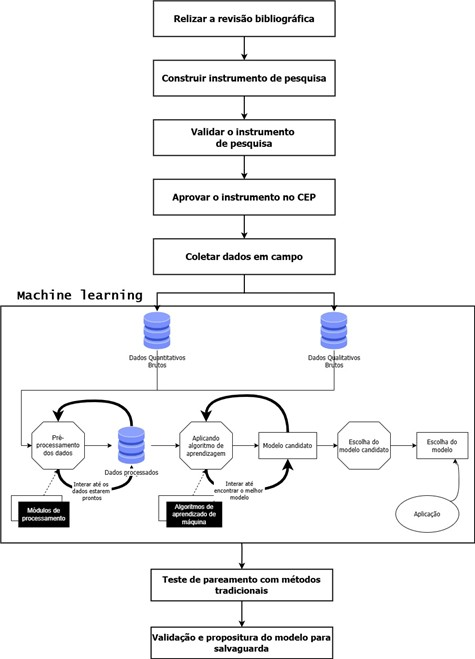
\includegraphics[scale=1.8]{Imagens/fig_2.pdf}
  \fonte{\textbf{Elaborado pelos autores} (2022)}
  \label{fig:2}
\end{figure}
\end{landscape}

Por fim, é importante ressaltar que a avaliação da metodologia proposta neste estudo está mediada pela técnica desenvolvida por \citeonline{Costa2015a}, tendo como base a \textit{Assessment of Multiple Systematic Reviews} (AMSTAR).

%%%%%%%%%%%%%%%%%%%%% Métodologia questionário%%%%%%%%%%%%%%%%%%%%%%%

\subsubsection*{Análise dos dados textuais selecionados}

\subsubsection*{\textit{Análise quantitativa dos dados textuais}}

Após a seleção dos comentários diretamente relacionados ao tema proposto nesta pesquisa, foram realizadas lexicométricas e análises de discursos nos textos presentes com o auxílio do software IRaMuTeQ \cite{Paulovich2008,DaSilvaCezar2018}. Através da utilização de Unidades de Contexto Iniciais (UCIs) na construção do modelo para análise, foi realizada uma prévia correção no conjunto de dados brutos, mantendo as palavras analisáveis, os termos caracterizados como substantivos, adjetivos e verbos. As palavras que geralmente não são relevantes para uma análise, como preposições e advérbios, foram excluídas.

Ao se trabalhar com corpus textuais, cada conjunto de texto deve compor uma UCI. Um conjunto de UCI é conhecido como corpus de análise, que o software segmenta em textos de aproximadamente três linhas, chamados Segmentos de Texto (ST) \cite{Fernandes2018ManualPortuges}. 

\subsubsection*{\textit{Análise qualitativa dos dados}}

Após a segmentação dos textos, foi realizada uma Classificação Hierárquica Descendente (CHD) dando origem a classes lexicais caracterizadas pelo vocabulário e a segmentos de textos que partilham o mesmo vocábulo. A CHD consiste em uma categoria de análise de conglomerado que categoriza as palavras obtidas em classes lexicais (eixos). A análise avalia a constância e os arranjos das palavras ativas no \textit{corpus} textual usando os dados das tabelas de contingência das palavras existentes \cite{Mendes2019,Carvalho2020a}. 

Neste sentido, as diferentes classes resultantes representam o espaço de sentido das palavras narradas, surgindo, assim, elementos pertencentes aos temas observáveis da pesquisa \cite{Gavasso2016}.


\subsection{Amostra utilizada}

Como fonte de dados realizou-se entrevistas com proprietários de 8 (oito) marcas de produtos amazônicos\footnote{\href{https://empreendasustentavel.com/index_2.html}{\color{blue}{\underline{Neste link é possível saber mais sobre as marcas utilizadas}}}}, que desenvolvem seus produtos considerando a sustentabilidade florestal. O estudo concentrou-se em 6 cadeias socioprodutivas da região: Turismo, Gastronomia, Biotecnologia, Sistemas Agroflorestais, Produtos Florestais Não Madeireiros e Moda Sustentável. 

\begin{figure}[H]
\centering
\caption{Marcas estudadas na pesquisa}
\subfigure[Logo Maha Biocosméticos]{

\includegraphics[scale=0.6]{Imagens/logo_mahabio.pdf}
\label{fig:27}
}
\subfigure[Logo De Mendes]{

\includegraphics[scale=0.6]{Imagens/logo_de_mendes.pdf}
\label{fig:28}
}
\subfigure[Logo UIKA]{

\includegraphics[scale=0.6]{Imagens/logo_uika.pdf}
\label{fig:28}
}
\subfigure[Logo Fazenda Bacuri]{

\includegraphics[scale=0.6]{Imagens/logo_fazenda_bacuri.pdf}
\label{fig:28}
}
\subfigure[Logo Muriki cicloturismo]{

\includegraphics[scale=0.6]{Imagens/logo_muriki.pdf}
\label{fig:28}
}
\subfigure[Logo Osaqui]{

\includegraphics[scale=0.6]{Imagens/logo_osaqui.pdf}
\label{fig:28}
}
\subfigure[Logo cogumelos Santa Bárbara]{

\includegraphics[scale=0.6]{Imagens/logo_santa_barbara.pdf}
\label{fig:28}
}
\subfigure[Logo Xibé]{

\includegraphics[scale=0.6]{Imagens/logo_xibe.pdf}
\label{fig:28}
}
%\fonte{\citeonline{Mendes2020ChocolateMendes}}
\end{figure}


\subsubsection{Descrição das marcas analisadas}



\subsubsubsection*{De Mendes Chocolates}

Atendendo à cadeia de alimentos, foi utiliza da empresa Chocolates De Mendes. Neste estudo, buscou-se analisar a marca de Chocolates De Mendes a partir de seus produtos, site, embalagens e apresentação do empreendedor.

A empresa é inserida na comunidade tradicional de Colônia Chicano, em Santa Bárbara, na região metropolitana de Belém do Pará, a empresa é reconhecida pela qualidade e pelos sabores diferenciados de suas barras de chocolate, oriundos do uso responsável e sustentável de recursos naturais da Amazônia, bem como da colaboração com as populações locais.

O fundador \citeonline{Mendes2020ChocolateMendes} cita que, a fundação da Chocolates De Mendes em 2014 reflete o comprometimento como empreendedor em estabelecer uma cadeia produtiva sustentável, em harmonia com as populações tradicionais da Amazônia, como indígenas, quilombolas, ribeirinhos, caboclos e agricultores familiares. Valorizando a cultura e o \textit{savoir-faire} desses povos, a produção dos chocolates é totalmente artesanal e fundamentada na seleção criteriosa de cacau nativo de excelência sensorial.


\begin{figure}[H]
\centering
\subfigure[Biscoito de castanha do Pará com puxuri]{

\includegraphics[scale=0.4]{Imagens/fig_27.pdf}
\label{fig:27}
}
\subfigure[Barra de chocolate Acará-Açu]{

\includegraphics[scale=0.4]{Imagens/fig_28.pdf}
\label{fig:28}
}
\caption{Produtos comercializados pela De Mendes Chocolates}
\fonte{\citeonline{Mendes2020ChocolateMendes}}
\end{figure}

Neste contexto, a empresa De Mendez Chocolates ilustra para este estudo o potencial da diversidade de recursos da Amazônia no desenvolvimento de produtos alimentícios, como chocolates. Ao compreender a complexidade dos recursos naturais e o envolvimento com as comunidades tradicionais locais a partir do trabalho colaborativo com comunidades locais, capacitando-as para o fornecimento de amêndoas de cacau e cupuaçu, seguindo padrões rigorosos de qualidade e sustentabilidade ambiental. Promovendo assim uma  abordagem inovadora para capitalização de matéria-prima, a marca De Mendez Chocolates fomenta o crescimento de novas produtos inseridos na cadeia produtiva de alimentos sustentáveis na região amazônica. 

Como representação simbólica, a marca utiliza em sua logo o símbolo de um fruto de cacau pintado com uma tonalidade terrosa, um aceno direto à origem natural dos produtos. O fruto de cacau é detalhado, apresentando uma textura realista que sugere uma sensação tátil, reforçando a ligação do consumidor com a natureza.

A tipografia não serifada DE MENDES aparece logo abaixo do fruto de cacau. O texto é exibido em uma cor azul rica e profunda que contrasta com o marrom terroso do cacau, proporcionando um equilíbrio visual ao logo. A escolha da fonte sem serifa acrescenta uma estética moderna e minimalista ao design, tornando a marca facilmente legível e distinguível.

O contraste entre o fruto de cacau terroso e a tipografia azul ajuda a enfatizar a mensagem de equilíbrio que a marca De Mendes quer transmitir - um equilíbrio entre tradição e modernidade, entre natureza e cultura, entre o exótico e o familiar. Ao todo, este logo transmite a imagem de uma marca sofisticada, que respeita as suas raízes e, ao mesmo tempo, busca constantemente inovação \cite{Mendes2020ChocolateMendes}.


\subsubsubsection*{Fazenda Bacuri e Produtos Osaqui}

A Fazenda Bacuri é uma agroempresa familiar localizada no município de Augusto Corrêa, na região nordeste do Estado do Pará, na Amazônia Oriental. Com origem nos anos 70 por Henrique Osaqui, um economista nipo-brasileiro, a companhia produz o bacuri, fruto típico da biodiversidade amazônica. Utilizando sistemas de manejo orgânico por rebrotamento natural do bacurizeiro (\textit{Platonia insignis}) e trabalhando com Sistemas Agroflorestais envolvendo outras culturas, a Fazenda Bacuri atua no desenvolvimento sustentável da região \cite{Bacuri2023FazendaBacuri}.

Além da produção de bacuri, a Fazenda Bacuri desenvolve uma linha de produtos que se baseia em alimentos e bebidas, como geleias, licores e frutas secas (Figura \ref{fig:29} e \ref{fig:26}). Todos os produtos são provenientes de sistemas de manejo agroflorestal orgânico certificado, implementado pelo fundador Henrique Osaqui desde 1970. A fazenda também atua no turismo rural, participando do roteiro Rota Amazônia Atlântica e promovendo a bioeconomia da floresta em pé em parceria com outras atividades agrícolas e de pesca locais \cite{Bacuri2023FazendaBacuri}.

\begin{figure}[H]
\centering
\subfigure[Fruta seca bacuri]{

\includegraphics[scale=0.25]{Imagens/fig_29.pdf}
\label{fig:29}
}
\subfigure[Licor de Genipapo]{

\includegraphics[scale=0.25]{Imagens/fig_26.pdf}
\label{fig:26}}
\caption{Produtos comercializados pela marca Osaqui}
\fonte{\citeonline{Bacuri2023FazendaBacuri}}
\end{figure}

Com a inauguração da Agroindústria Familiar em 2014 e o lançamento de produtos com certificação 100\% orgânica, a Fazenda Bacuri iniciou seu compromisso com a sustentabilidade e a preservação dos recursos naturais. O projeto de turismo rural "Rota Amazônia Atlântica", iniciado em 2015, contribui ainda mais para a valorização do patrimônio ecológico e cultural da Amazônia, gerando oportunidades para o fortalecimento e a ampliação de iniciativas sustentáveis na região \cite{MinisteriodoTurismo2021ProjetoBacuri}.

Nesse contexto, a Fazenda Bacuri exemplifica para esta pesquisa o vasto potencial inexplorado das práticas sustentáveis e do ecoturismo na região amazônica. Ao engajar-se em atividades diversificadas, como manutenção de agroflorestas, meliponicultura, sistemas agroflorestais, agroindústria e turismo rural, a Fazenda Bacuri promove um modelo empresarial multifacetado e ambientalmente consciente.

Quanto a logomarca da Fazenda bacuri, esta representa as árvores bacurizeiros presentes na reserva que nomeia a fazenda e seguem em harmonia com a fonte cursiva.

\subsubsubsection*{UIKA turismo comunitário}

A UIKA se constitui como uma startup operadora de turismo florestal, cujo objetivo principal é prover turismo comunitário na região amazônica, priorizando a cultura amazônica e os empreendedores locais \cite{UIKA2023UIKAAmazonia}. Dentre as ofertas proporcionadas pela UIKA estão experiências imersivas em comunidades ribeirinhas e indígenas, roteiros históricos, culturais e gastronômicos em Manaus, viagens fluviais pelos rios amazônicos e interação ímpar com a natureza \cite{UIKA2023UIKAAmazonia}.

\begin{figure}[H]
\centering
\subfigure[Artesanatos comercializados pelas comunidades traducionais]{

\includegraphics[scale=0.4]{Imagens/fig_30.pdf}
\label{fig:27}
}
\subfigure[Comunidades ribeirinhas-AM]{

\includegraphics[scale=0.17]{Imagens/fig_31.pdf}
\label{fig:28}}
\caption{Experiências turísticas promovidas pela UIKA}
\fonte{\citeonline{UIKA2023UIKAAmazonia}}
\end{figure}

O termo UIKA origina-se da língua indígena Kambeba, significando um habitante fronteiriço, que vive em um local onde se avistam dois mundos, mas que tem o olhar voltado ao desconhecido, ou seja, remete à figura do viajante. A UIKA surgiu como resultado de um sonho coletivo no coração da floresta amazônica, fruto do desejo de que os amazônidas se tornem protagonistas de suas histórias e compartilhem seus conhecimentos e habilidades com o mundo sob a perspectiva de alguém que nasceu e cresceu na região.

A fundação da UIKA se originou a partir de uma consultoria na área de turismo comunitário na comunidade indígena Três Unidos, localizada a 60 km de Manaus no Rio Cuieiras, onde foi batizada com o nome UIKA por um jovem Kambeba chamado Muipiruata \cite{UIKA2023UIKAAmazonia}.

Assim sendo, a empresa UIKA exemplifica para este estudo o potencial latente da região amazônica no desenvolvimento de novos empreendimentos turísticos focados na criatividade e no capital intelectual. Ao abraçar a riqueza histórica, social e cultural da Amazônia e promover abordagens inovadoras para o uso sustentável desses elementos, a marca UIKA contribui para o impulso do desenvolvimento socioeconômico por meio do turismo sustentável na região amazônica.


A logomarca da UIKA busca representar em suas cores e textura o por do sol, símbolo da capital Manaus, do estado Amazonas.


\subsubsubsection*{Muriki Cicloturismo}

A Muriki Cicloturismo é uma empresa de turismo de aventura em cicloturismo que oferece passeios pela região de Santarém e Alter do Chão na Amazônia \cite{Muriki2023MurikiCicloturismo}.
Com sua  base em Santarém, no Oeste do Pará \cite{IBGE2023DadosSantarem}. A cidade de Santarém, é conhecida como a "Pérola dos Tapajós" e é uma das principais potências do turismo natural do Estado \cite{PortalAmazonia2023PerolaAmazonia}.

A estruturação dos roteiros promovidos pela Muriki pretende promover uma compreensão mais profunda da exuberância e diversidade da Floresta Amazônica, permitindo isso com um alto nível de conforto, segurança e uma ética de responsabilidade ambiental \cite{Muriki2023MurikiCicloturismo}. Os participantes da experiência serão levados por uma variedade de ambientes naturais, incluindo praias fluviais, trilhas ecológicas (Figura \ref{fig:32}), córregos menores denominados "igarapés" (Figura \ref{fig:33}), comunidades indígenas e tradicionais (Figura \ref{fig:34}), assim como eventos esportivos e corridas ciclísticas (Figura \ref{fig:35}). Além disso, projetos de manejo florestal comunitário estarão presentes ao longo dos roteiros, fornecendo um panorama mais completo da vida na região.

A experiência promovida pela Muriki também abarca um entendimento mais amplo da cultura local. Os participantes vivenciam a interação com a gastronomia, o artesanato local e serão introduzidos à rica fauna e flora da região, que possui a maior biodiversidade do planeta.

A interação com a Floresta Amazônica proporcionada pelo turismo de Cicloturismo, além de ser uma experiência enriquecedora, cultural, possui um papel fundamental na conscientização e na promoção da sustentabilidade ambiental. A vivência turística na Amazônia, em particular, pode ser um catalisador para o entendimento e a valorização da biodiversidade local, a qual é de importância global \cite{Rafa2021EcotourismBangladesh}. A partir do cicloturismo comunitário, os participantes são incentivados a interagir com a floresta de uma maneira respeitosa e consciente, compreendendo a importância de preservar essa incrível reserva de biodiversidade para as futuras gerações \cite{Ciascai2022CyclingPerspectives}.

\begin{figure}[H]
\centering
\subfigure[Trilhas ecológicas]{

\includegraphics[scale=1.7]{Imagens/fig_32.pdf}
\label{fig:32}
}
\subfigure[Experiências locais]{

\includegraphics[scale=0.4]{Imagens/fig_34.pdf}
\label{fig:33}
}
\subfigure[Experiências comunitárias]{

\includegraphics[scale=0.4]{Imagens/fig_35.pdf}
\label{fig:34}
}
\subfigure[Eventos esportivos]{

\includegraphics[scale=1.3]{Imagens/fig_33.pdf}
\label{fig:35}
}
\caption{Experiências ciclo turísticas promovidas pela Muriki}
\fonte{\citeonline{Muriki2023MurikiCicloturismo}}
\end{figure}


A Muriki Cicloturismo oferece uma variedade de roteiros adaptados a diferentes preferências e níveis de habilidade. Isso vai desde excursões de um único dia até expedições de vários dias pela Floresta Nacional do Tapajós, uma das áreas mais preservadas e impressionantes da Amazônia \cite{Ciascai2022CyclingPerspectives}. Quanto ao perfil de responsabilidade ambiental sustentável, a empresa adota um enfoque de turismo responsável que, além de minimizar o impacto ambiental de suas atividades, também contribui para a preservação e valorização dos ecossistemas locais.

Conforme essa perspectiva, a empresa Muriki Cicloturismo ilustra para este estudo o potencial latente da região amazônica no desenvolvimento de novas atividades ecoturísticas, como o cicloturismo florestal. Ao compreender a complexidade dos ecossistemas locais e implementar estratégias inovadoras para o uso sustentável desses recursos, a marca Muriki Cicloturismo colabora para o crescimento de novos empreendimentos relacionados à cadeia do ecoturismo sustentável na região amazônica \cite{Ciascai2022CyclingPerspectives}.

A nome Muriqui é uma denominação comum as duas espécies de macacos do Novo Mundo da família \textit{Atelidae} e gênero \textit{Brachyteles} também conhecidos como buriquins \cite{Melo2004NovosBahia}. É o maior macaco americano, medindo 0,70 metros de corpo e igual medida de cauda. Tem polegar reduzido e pelo amarelo. Vive nas matas dos estados de São Paulo, Rio de Janeiro, Minas Gerais e Espírito Santo, nos fragmentos de mata atlântica que restam nestes estados do Brasil \cite{Aximoff2015ConfirmacaoBrasil}.

\subsubsubsection*{Xibé}

A indústria da moda é uma das maiores poluentes do mundo e, nos últimos anos, a preocupação com a sustentabilidade e o consumo consciente tem crescido exponencialmente, influenciando o mercado da moda \cite{Pucker2022TheFashion}. Nos últimos anos, houve um ressurgimento no interesse pela aplicação de corantes naturais na tinturaria de materiais têxteis, em parte devido à conscientização ambiental e ao desejo de produtos naturais e sustentáveis \cite{Kumar2020FundamentalsSubstrates}. 


Nesse contexto, a startup Xibé foi selecionada com um enfoque na moda sustentável, produção e comercialização de produtos de tinturaria e confecção a partir de recursos naturais da Amazônia, visando reduzir seu impacto ambiental. 

A Xibé possui uma linha de produtos que incluem tintas naturais (Figura \ref{fig:36}), lenços pashmina (Figura \ref{fig:37}), blusas e bolsas (Figura \ref{fig:38}), todos confeccionados e tingidos de maneira sustentável a partir de fontes naturais amazônicas \cite{Kumar2014SustainabilityPerspective}. Os corantes naturais da Xibé representam uma alternativa ecologicamente viável aos corantes sintéticos tradicionalmente utilizados na indústria têxtil, responsáveis por grande parte da poluição gerada pelo setor \cite{Pucker2022TheFashion}.


\begin{figure}[H]
\centering
\subfigure[Tinturas naturais desenvolvidas pela Xibé]{

\includegraphics[scale=0.15]{Imagens/fig_36.pdf}
\label{fig:36}
}
\subfigure[Lenços pashmina Xibé]{

\includegraphics[scale=0.15]{Imagens/fig_37.pdf}
\label{fig:37}
}
\subfigure[Acessórios artesanais comercializados]{

\includegraphics[scale=0.15]{Imagens/fig_38.pdf}
\label{fig:38}
}
\subfigure[Bolsas desenvolvidas pela Xibé]{

\includegraphics[scale=0.15]{Imagens/fig_39.pdf}
\label{fig:39}
}
\caption{Experiências ciclo turísticas promovidas pela Muriki}
\fonte{\citeonline{Muriki2023MurikiCicloturismo}}
\end{figure}

Neste contexto, a startup Xibé surge como um exemplo significativo para esta investigação, representando o potencial ainda não explorado dos recursos da biodiversidade amazônica no desenvolvimento de corantes naturais e produtos têxteis ecológicos. Ao compreender a complexidade dos elementos naturais presentes na região e fomentar abordagens inovadoras para o aproveitamento destes, a marca Xibé contribui para a criação de novas iniciativas e marcas no âmbito da indústria da moda sustentável na região amazônica.

Quanto ao nome, Xibé é um palavra em tupo que representa um alimento originário de uma raiz indígena, consumido na região amazônica. Uma mistura de água com farinha de mandioca que pode ser degustado puro ou com pirarucu e outros peixes, fritos ou assados, como também charque.

\subsubsubsection*{Cogumelos Santa Bárbara}

A Amazônia é uma região de vasta riqueza, abrangendo um mosaico de ingredientes e culturas únicas. Dentre seus aportes ao mercado mundial, os cogumelos amazônicos comestíveis representam uma fonte relevante de nutrientes e um nicho promissor para o empreendedorismo sustentável. Ressurge sob esse contexto a Cogumelos Santa Bárbara, uma startup voltada à produção e comercialização de cogumelos amazônicos comestíveis, que busca aliar inovação e sustentabilidade regional.

Localizada na cidade homônima do Estado do Pará, a Cogumelos Santa Bárbara desenvolve suas atividades visando ao equilíbrio socioambiental e produtivo ao seu negócio. A empresa opera de forma responsável, respeitando a série de exigências legais e éticas, que permeiam uma produção regenerativa e alinhada à conservação da biodiversidade local \cite{CogumelosSantaBarbara2023CogumelosBarbara}. A startup promove o cultivo de diversas espécies de cogumelos comestíveis amazônicos e exóticos, fomentando biomercado com sabor regional e agregando valor nutricional a seus produtos.

A Cogumelos Santa Bárbara adota práticas sustentáveis, desde o processo de cultivo utilizando  caroços do açaí como substrato, até a logística de distribuição de seus produtos \citeonline{CogumelosSantaBarbara2023CogumelosBarbara}. A empresa utiliza técnicas agrícolas ambientalmente responsáveis, como a integração entre produção agroflorestal e cogumelos, diversificando a matriz produtiva amazônica e estimulando outras modalidades de renda para as comunidades locais. A startup preza pelo apoio constante ao manejo sustentável dos recursos naturais e pela valorização dos aspectos culturais da região, gerando oportunidades de emprego e distribuição de renda.

No que diz respeito aos resíduos gerados durante a produção, a empresa adota políticas de redução, reutilização e reciclagem, aproveitando ao máximo os nutrientes e resíduos dos processos produtivos. Emissões de carbono, consumo de energia e de água são minimizados durante todo o processo, e o tratamento de efluentes é realizado de forma responsável, já que a startup utiliza pequenos espaços para sua estufa, utilizando pouca energia elétrica para manutenção da temperatura interna, apenas para circulação de ar interno (Figura \ref{fig:44}).

\begin{figure}[H]
\centering
\subfigure[Visão interna da estufa]{

\includegraphics[scale=0.2]{Imagens/fig_43.pdf}
\label{fig:44}
}
\subfigure[Visão externa da estufa]{

\includegraphics[scale=0.2]{Imagens/fig_44.pdf}
\label{fig:44}
}
\caption{Estufas Cogumelos Santa Bárbara}
\fonte{\citeonline{CogumelosSantaBarbara2023CogumelosBarbara}}
\end{figure}


A startup Cogumelos Santa Bárbara emerge como um exemplo significativo nesta investigação, evidenciando o potencial inexplorado dos recursos da biodiversidade amazônica no desenvolvimento e comercialização de cogumelos regionais destinados ao consumo alimentar. Ao valorizar a identidade amazônica e empregar práticas sustentáveis no cultivo de cogumelos, a marca Cogumelos Santa Bárbara contribui para a criação de novas iniciativas e marcas no setor alimentício responsável e alinhado à preservação da região.

A estratégia de \textit{Branding} adotada pela Cogumelos Santa Bárbara visa ressaltar o seu compromisso socioambiental, comunicando aos consumidores que seus produtos são saudáveis, diferenciados, cultivados de maneira orgânica e com respeito ao bioma e às comunidades locais. A posição de mercado da empresa é direcionada a um público criterioso e consciente, interessado em alimentos de origem orgânica, amazônicos e com alto valor nutricional.

Mantendo um diálogo aberto e transparente com sua base de clientes, a startup promove ações e campanhas de conscientização sobre o consumo responsável e a importância da conservação da biodiversidade amazônica. Desse modo, Cogumelos Santa Bárbara demonstra o papel fundamental do empreendedorismo sustentável e das estratégias de \textit{Branding} eficazes no fortalecimento das práticas sustentáveis e na valorização dos recursos da região amazônica.


\subsubsubsection*{Mahabio biocosméticos}

Atualmente, o mercado de cosméticos está focado em organizar práticas sustentáveis e promover o uso de recursos naturais em seus produtos. A demanda por cosméticos eco-eficientes tem levado empresas a explorar alternativas naturais e recursos da biodiversidade mundial (Jones et al., 2016). A região amazônica é reconhecida por sua biodiversidade única e oferece uma rica variedade de recursos naturais, substâncias bioativas e vegetais que pode ser aproveitada para o desenvolvimento de novos produtos cosméticos (Ferreira et al., 2017). 

Dentro deste cenário, selecionamos a startup Mahabio como um estudo de caso para enquadrar o desenvolvimento e comercialização de uma gama de produtos cosméticos inovadores à base de substratos amazônicos naturais, incluindo o condicionador de andiroba, xampu com base em castanha-do-pará e creme de ucuuba. Os produtos desenvolvidos pela Mahabio consistem em: 


1. Condicionador de Andiroba (Figura \subref{fig:40}): a andiroba (\textit{Carapa guianensis}) é uma árvore da Amazônia cujo óleo é conhecido por suas propriedades anti-inflamatórias, cicatrizantes e inseticidas \cite{MartinsCunhaJunior2021BrazilianActivity}. A Mahabio formulou um condicionador com base nesse óleo, oferecendo uma opção natural e sustentável para cuidado e tratamento capilar.

2. Xampu de Castanha-do-Pará (Figura \subref{fig:41}): a castanha-do-pará (\textit{Bertholletia excelsa}) é uma semente amazônica conhecida por seus nutrientes e propriedades antioxidantes \cite{WadtSustainablePopulations}. A Mahabio incorpora o óleo de castanha-do-pará em um xampu de alta qualidade, oferecendo o melhor em termos de nutrição e proteção capilar.

3. Creme de Ucuuba (Figura \subref{fig:42}): a ucuuba (\textit{Virola sebifera}) é uma árvore amazônica rica em manteiga vegetal com propriedades hidratantes, cicatrizantes e anti-inflamatórias \cite{Modesto2022CaracterizacaoWarb./em}. A Mahabio utiliza a manteiga de ucuuba como ingrediente principal em seu creme, garantindo uma hidratação profunda e regeneração da pele.



\begin{figure}[H]
\centering
\subfigure[Condicionador de Andiroba]{

\includegraphics[scale=0.2]{Imagens/fig_40.pdf}
\label{fig:40}
}
\subfigure[Xampu de Castanha-do-Pará]{

\includegraphics[scale=0.2]{Imagens/fig_41.pdf}
\label{fig:41}
}
\subfigure[Creme de Ucuuba]{

\includegraphics[scale=0.2]{Imagens/fig_42.pdf}
\label{fig:42}
}
\caption{Produtos desenvolvidos pela Mahabio}
\fonte{\citeonline{Muriki2023MurikiCicloturismo}}
\end{figure}


Neste sentido, a startup Mahabio exemplifica para esta pesquisa o potencial inexplorado da biodiversidade amazônica no desenvolvimento de novos produtos cosméticos. Ao reconhecer a complexidade dos recursos naturais e promover técnicas inovadoras para a utilização desses recursos, a marca Mahabio contribui para o desenvolvimento de novas marcas relacionadas a cadeia cosmética sustentável na região amazônica.


%%%%%CAPÍTULO 2
\subsection{Instrumentos para análise dos elementos de \textit{Brand Equity}}

\subsubsection{Surveys utilizados}

A segunda fase metodológica é caracterizada pelo desenvolvimento de dois \textit{surveys}.

Na primeira fase, buscando compreender a percepção dos empreendedores a partir do seu modelo de negócio relacionado à conexão da marca Amazônia, foi elaborado um roteiro de entrevista semiestruturado (Apêndice B) proposto para os empreendedores. 

Na segunda fase, objetivando verificar quais os elementos de design gráfico na identidade aplicada na marca influenciam as motivações das escolhas dos consumidores pelos produtos e identificar quais os valores atribuídos à marca sustentabilidade ambiental da Amazônia brasileira influenciam a preferência na aquisição do produto, foi desenvolvido um instrumento inicial (Apêndice C). Objetiva-se compreender a percepção e os níveis de satisfação associados os valores adicionais (\textit{Brand Equity}) presentes nas marcas empresariais relacionadas à sustentabilidade ambiental na região da amazônia do Brasil. 

Ao considerar o atual momento pandêmico e a abrangência populacional adotada, optou-se por realizar uma pesquisa on-line. Consoante a \citeonline{Walter2016}, devido às suas vantagens, como velocidade e capacidade, as pesquisas on-line estão cada vez mais sendo utilizadas por pesquisadores para atingir populações específicas, reduzindo possíveis custos.

\subsubsection*{\textit{Questionário para os empreendedores}}

As entrevistas com os proprietários das marcas foram realizadas por videochamada no período de 15 de fevereiro de 2022 a 16 de junho de 2022. O instrumento inicial teve como base as dimensões da sustentabilidade propostas por \citeonline{Sachs2002CaminhosSustentavel}. Para as dimensões: econômica (fonte de matéria-prima, produtos etc.), social (paridade, masculino feminino, conscientização de comunidades locais etc.) e ambiental (redução de embalagens, redução das emissões de $C0_2$ etc.) foi adaptado o questionário proposto por \citeonline{Postel2006LaFordiste} \textit{Triple Bottom Line}. As dimensões: cultural, ecológica, territorial, política (nacional) e política (internacional) foram avaliadas utilizando adaptações do questionário proposto por \cite{Grigorescu2019KeySustainability}


\subsubsection*{Questionário para consumidores}

Buscando contemplar os dados quali-quantitativos da percepção dos consumidores, nesta pesquisa, foi adaptada uma ferramenta de coleta de dados contendo cinco blocos de construtos:

O pré-teste de identificação, o qual foi composto por cinco questões que buscam traçar o perfil dos entrevistados, levantando informações tais como: sexo, faixa etária, região geográfica residente, faixa socioeconômica, conhecimento da existência do programa Amazônia UP. 

O \textbf{Primeira dimensão} foi composto por onze questões, que avaliaram a percepção do entrevistado sobre a relevância da sustentabilidade ambiental na região amazônica do Brasil e o nível de percepção dos participantes quanto à importância da relação da empresa ou \textit{startup} com a sustentabilidade ambiental na região  \cite{Grigorescu2019KeySustainability}. Inicialmente, ele foi composto tendo como base 12 questões. Para tanto, as questões do construto foram divididas em dois blocos. 

Um primeiro bloco foi solicitado aos entrevistados que avaliaram o grau em que percebem cada marca como uma marca de baixo ou alto nível de envolvimento com políticas de sustentabilidade ambiental por meio da descrição do propósito e o portfólio constantes das marcas, esta pontuação contou com  5 questões com uma escala de cinco pontos. Este bloco avaliou o posicionamento estratégico da marca (\textit{Strategic brand positioning} - SBP) na região amazônica do Brasil. A dimensão foi composta inicialmente por 10 (dez) questões transliteradas da escala desenvolvida por \citeonline{Grigorescu2019KeySustainability}.

Já o \textbf{Segunda dimensão} apresentou 5 (cinco) itens e compreendeu a percepção da qualidade do produto (\textit{Brand quality perception} - BQP) e o valor da marca relacionado à sustentabilidade ambiental propostos inicialmente por cada marca. Este construto foi composto por 5 figuras/itens da marca, 5 imagens da loja (digital ou física), 5 figuras de outros produtos e quatro figuras/itens do produto \textit{premium} (com valor acima da média do mercado) e 5 figuras que representem a intenção empresarial frente à sustentabilidade ambiental da Amazônia (meio de produção/extração). De mãos das figuras/produtos. Os cinco itens foram adaptados dos instrumentos desenvolvidos por \citeonline{Netemeyer_Krishnan} e \citeonline{Yoo2017AnEquity:}.

Já o \textbf{Terceira dimensão} contendo inicialmente 5 (cinco) questões, que buscam compreender a que os participantes estariam dispostos para adquirir os produtos advindos das marcas relacionadas à sustentabilidade ambiental da floresta (\textit{Purchase Intention} - PI). Para medir a intenção de compra, foram adaptados três itens dispostos no trabalho de \citeonline{Arnett-meiers}, já para avaliar a disposição de pagar um preço \textit{premium}, quatro itens de \citeonline{Netemeyer_Krishnan}.

O \textbf{Quarta dimensão} avaliou o quanto o negócio apresenta inovação em seu \textit{Branding} (\textit{Retail Innovation} - RI). O construto foi composto por 5 questões que abordam o tema inovação e design.

Para que esta fase não resultasse em cansaço físico dos participantes por visualização excessiva, as imagens foram criteriosamente selecionadas e categorizadas em 5 grupos, em que cada participante da pesquisa só visualizaria 3 grupos com 3 \textit{startups}, fracionando assim as demais em quantidades iguais na população pesquisada.

Buscando atender aos princípios éticos em pesquisas com seres humanos, o presente estudo foi encaminhado ao Comitê de Ética em pesquisa da Universidade Federal de Sergipe. Os participantes que aceitarem a participação no estudo foram esclarecidos quanto aos objetivos, à coleta de dados, bem como, às informações contidas no Termo de Consentimento Livre e Esclarecido (TCLE).


- SBP = Strategic brand positioning
- BQP = Brand quality perception
- BA = Brand authenticity
- PI = Purchase Intention
- RI = Retail Innovation


\subsubsection*{\textit{Protocolo de validação dos instrumentos}}

Após a formulação e estruturação dos itens a serem utilizados no instrumento de coleta de dados, este foi submetido à validação com base no modelo tripartite, descrito no \textit{Standards for Educational and Psychological Testing} \cite{Association2018}, que apresenta o processo de validação nas seguintes fases: 

\begin{enumerate}
- Validação de conteúdo; 
- Validade baseada na estrutura interna; 
- Validade baseada nas relações com medidas externas; 
- Validade baseada no padrão de resposta aos itens e
- Validade consequencial.
\end{enumerate}

\subsubsection*{\textit{Validade de conteúdo}}

Para medir a eficácia do questionário proposto neste estudo, o método Coeficiente de Validade de Conteúdo (CVC) foi utilizado como parâmetro de verificação. Essa técnica envolve a busca do bom senso de uma comunidade de juízes (ou seja, profissionais efetivamente envolvidos na área de pesquisa). O método CVC baseia-se na aplicação estruturada do conhecimento e da experiência de especialistas da área, pressupondo que o julgamento conjunto de um determinado processo, se bem organizado, é melhor que a opinião de uma única pessoa \cite{Santos2018,Gurgel2021}.

O CVC é uma técnica quantitativa em que se calcula a concordância que juízes distintos possuem sobre um mesmo instrumento. Habitualmente, isso é feito solicitando que eles atribuam um valor gradual (1 a 5) aos itens, em função da clareza da linguagem de cada item (a quão clara e compreensível está a sentença), pertinência (o quanto o item é pertinente para analisar a dimensão analisada) e relevância (o quanto ele pode discriminar o construto e o quanto é relevante para a medida).  Após isso, basta aplicar a equação \ref{eq:1}:

\begin{equation}
CVC_{i}=\frac{k}{j}*\left (\frac{\sum_{i}=1x_{i}}{E}\right)
\label{eq:1}
\end{equation}

- Em que: (K) é o número de itens; - (Xi) é cada item
- (J) é o número de juízes
- (E) é o número de itens da escala (questionário).

De modo que o resultado de CVC foi obtido pela Equação \ref{eq:2}:

\begin{equation}
CVC=\frac{1}{N}*CVC_{i}
\label{eq:2} 
\end{equation}

Onde: (N) é o número de itens.

Por fim, foi solicitado a cada juiz se houve necessidades de modificação do item. A avaliação do questionário pelos juízes foi realizada às cegas, portanto, acreditou-se que a confidencialidade dos participantes garantiu maior fidelidade aos resultados ao final do experimento e permite uma melhor exposição, além de manter a sua compreensão do questionário proposto \cite{Hasson2000}.

\subsubsection*{\textit{Validade baseada na estrutura interna}}

A validade baseada na estrutura interna reflete o grau onde a estrutura de correlações entre os itens está conforme o construto que o teste se propõe a medir \cite{Association2018}. As variáveis latentes ou construtos são fenômenos que não são diretamente observáveis, mas que podem ser inferidas através da relação entre variáveis observáveis, ou seja, que podem ser medidas diretamente, a exemplo dos itens de um instrumento \cite{Reckase2016}.

A análise fatorial é um método utilizado para investigar as relações entre as variáveis observáveis e, a quais fatores ou construtos elas se relacionam, possibilitando organizar muitas variáveis em um conjunto menor de fatores \cite{gonzalez2002}. 

Para tanto, nesta pesquisa, foi realizada uma Análise Fatorial Exploratória (AFE) para avaliar o comportamento estrutural da escala proposta. A análise foi implementada utilizando uma matriz policórica e, para o método de extração, utilizou-se do método \textit{Robust Diagonally Weighted Least Squares} (RDWLS) \cite{Asparouhov2010}. A decisão sobre o número de fatores a ser retido foi realizada por meio da técnica da Análise Paralela com permutação aleatória dos dados observados \cite{Timmerman2011}. 

Para determinar o número de fatores de retenção e facilitar a interpretação dos fatores \cite{Damasio2012}, foi adotado como método de rotação utilizado semelhante à oblíqua \textit{Robust Promin} \cite{Lorenzo-Seva2019}. O \textit{Robust Promim} objetiva obter uma matriz simples e estável em todas as amostras, ou seja, concentra-se em maximizar a simplicidade da solução rotacionada e nos valores de carregamento das variáveis, cujas correlações com as demais variáveis são as mais estáveis \cite{Lorenzo-Seva2019}.

Para avaliar a qualidade da adequação do modelo, de modo a aferir quão bem ele consegue reproduzir a estrutura de covariância ou a estrutura correlacional das variáveis, foram utilizadas as seguintes estratégias: raiz robusta do erro quadrático médio de aproximação (RMSEA), índice de Tuker-Lewis (TLI) e índice de ajustamento comparativo (CFI). Conforme a literatura \cite{Brown2015}, o valor de RMSEA deve ser menor que 0,08, o intervalo de confiança não pode chegar a 0.10. Os valores de CFI e TLI devem ser maiores que 0.90, preferencialmente 0.95.

A fiabilidade do modelo, ou seja, o quão consistente e reprodutível ele é em relação à medição das variáveis latentes pretendidas, foi testada a partir do indicador Fiabilidade Compósita, o qual deve apresentar valores maiores ou iguais a 0.70 \cite{Hair2009}.

A estabilidade dos fatores foi avaliada por meio do \textit{H-index} \cite{Ferrando2018AssessingAnalysis}. O \textit{H-index} avalia quão bem um conjunto de itens representa um fator comum \cite{Ferrando2017}. Os valores de H variam de 0 a 1. Valores altos de H (> 0.80) sugerem uma variável latente bem definida, provável que seja estável em diferentes estudos. Valores abaixo deste demonstram instabilidade entre diferentes estudos \cite{Ferrando2017}.
Por fim, o parâmetro de discriminação e os \textit{thresholds} dos itens foram avaliados utilizando a parametrização de \citeonline{Reckase2016}.

Para serem realizadas as análises estatísticas, foi utilizado o software SPSS \cite{Espessato2017}.

\subsubsection*{\textit{Validade baseada nas relações com medidas externas}}

Buscando avaliar a evidência de validade baseada na relação com outras variáveis dispostas em outros instrumentos \cite{Souza2017}, assim como a assimetria das informações deste.

\subsubsection*{\textit{Validade Convergente e discriminante}}

A validade convergente dos fatores foi avaliada através da variância média extraída (AVE), em que valores superiores a 0.50 são considerados indicativos de boa validade convergente \cite{Maroco2014}.
A validade discriminante dos fatores é aceita quando, para cada construto, a AVE for maior que o quadrado da correlação entre fatores \cite{Fornell1981EvaluatingError}.

\subsubsection*{\textit{Validade da Invariância das medidas}}

Buscando atender a esta validação, foi realizada uma Análise Fatorial Confirmatória Multi-grupo (AFCMG), buscando verificar a invariância das medidas do Modelo proposto em duas amostras selecionadas ao acaso na medida de 50\% para cada (T=Teste e A=Amostra) dos dados coletados.
AFCMG é uma técnica de modelagem de equações estruturais usada para avaliar o grau de invariância (equivalente) da configuração e dos parâmetros de uma determinada ferramenta psicométrica para diferentes grupos \cite{Sass2011}. Para cada grupo, foram testados três modelos de validade: 
 

- Invariância Configural;
- Invariância Métrica; 
- Invariância Escalar.


\citeonline{Borsa2018} explica que a Invariância Configural é um método utilizado para avaliar o grau de equivalência da estrutura fatorial da ferramenta para grupos diferentes (testa se a distribuição dos itens por fator ainda é suficientemente aceitável para amostras diferentes).

A invariância métrica avalia se as cargas fatoriais dos itens para grupos diferentes se mantêm, em outras palavras, avalia o grau em que os itens têm a mesma importância para a avaliação de estruturas em amostras diferentes. 

Por fim, a Invariância Escalar verifica se as pontuações obtidas estão totalmente relacionadas com o nível de traço latente dos sujeitos, independentemente do grupo a que pertençam, este teste é realizado estipulando que os interceptos dos itens para os diferentes grupos são iguais.

Para avaliar a invariância do questionário, foram utilizados os testes de diferença do \textit{Comparative Fit Index} ($\triangle$CFI) e a diferença por qui-quadrado. Para assumir a invariância da medida, em comparação com o modelo anterior, o índice de ajuste do modelo de teste no CFI não deve ser maior que 0.01 \cite{Cheung2002EvaluatingInvariance}, e para o valor do $\delta\chi^2$  deve apresentar um valor de p> 0.05 \cite{Milfont2010TestingResearch.}.

\subsubsection*{\textit{Validade de Critério Discriminante}}
\subsubsection*{\textit{Validade consequencial}}

O método de validade baseado em argumentação da consequência envolve exposição explicativa dos conteúdos e argumentação da validade inerente à hipótese buscada pela ferramenta, \cite{Kane2010}. O argumento explicativo especifica a interpretação proposta e o uso dos resultados do teste e estabelece uma rede de inferências e hipóteses a partir do desempenho observado até as conclusões e decisões baseadas no desempenho, \citeonline{Lane2014ValidityConsequences}

Este trabalho adotou como método de validação consequencial o delineamento adaptado de \citeonline{Zhang_J}:

\begin{enumerate}[label=\roman*]

- Relatar os efeitos pretendidos do sistema de avaliação.
- Descrever os componentes do sistema de avaliação, além de um fundamento lógico e coerente para cada componente, incluindo o apoio para esse fundamento teórico.
- As afirmações interpretativas feitas a partir dos resultados da avaliação.
- Os mecanismos de ação designados para causar os efeitos pretendidos.
\end{enumerate}

\subsubsection*{\textit{Validade baseada no padrão de resposta aos itens}}

Para validação baseada no padrão de respostas aos itens, esta validação foi adotada com os seguintes pressupostos:

\begin{enumerate}[label=\roman*.]
- Itens claros não geram desinteresse no ato de responder;
- Itens objetivos não geram respostas distantes do traço latente do avaliado;
- Questionário objetivo não gera cansaço exagerado ao responder.
\end{enumerate}


Buscando responder os pressupostos i e ii, foram avaliados por valores maiores que 0.70 ou, preferencialmente, valores maiores que 0.80 \cite{Linacre2012WinstepsGuide}. Os índices de \textit{infit} e \textit{outfit} quantificam resíduos para os itens em relação ao modelo testado \cite{Boone2016RaschHow}, \cite{Wright1994ReasonableTransactions}. foi adotado o índice de média quadrática ponderada, em inglês \textit{Weighted Mean-Squared Index} (WMSI), este índice é calculado usando valores limite ideais para detectar respostas potencialmente aberrantes \cite{Ferrando2017}.

Para responder o pressuposto iii, foi realizado também o \textit{person-fit índices for continuous models} de modo a observar se o banco de dados apresenta respostas de avaliados que não se esforçaram ao máximo para responder às perguntas do questionário, ou não realizaram o teste com a intenção de responder perguntas com o melhor de sua capacidade e que com isso apresentam \textit{outlier}. 


Foi realizado também o \textit{person-fit índices for continuous models}. Interessa-se observar a ocorrência se o banco de dados apresenta respostas de avaliados que não se esforçaram ao máximo para responder às perguntas do questionário ou não realizaram o teste com a intenção de responder às perguntas com o melhor de sua capacidade e que com isso apresentem \textit{outlier}.

\subsubsection*{\textit{Questionário proposto para percepção dos empreendedores locais}}

O questionário da entrevista semiestruturado proposto para os proprietários das marcas analisadas foi aplicado por videochamada no período de 15 de fevereiro de 2022 a 16 de junho de 2022. 

O instrumento inicial tem como base as dimensões da sustentabilidade propostas por \cite{Sachs2002CaminhosSustentavel}. Para as dimensões: econômica (fonte de matéria-prima, produtos, etc.), social (paridade da população com a comunidade local, conscientização de comunidades locais, etc.) e ambiental (redução de embalagens, redução das emissões de $CO_2$, etc.) foi adaptado o questionário proposto por \cite{Postel2006LaFordiste} \textit{Triple Bottom Line}. As dimensões: cultural, ecológica, territorial, política (nacional) e política (internacional) foram avaliadas utilizando adaptações do questionário proposto por \cite{Grigorescu2019KeySustainability}.


%%%%CAPÍTULO 3
\subsection{Interpretação dos construtos formadores da Fidelidade à marca e a qualidade percebida}

\subsubsection*{\textit{Modelo estrutural hipotético}}

Com base em estudos de revisão (Capítulo I), foi hipotetizada uma rede nomológica apresentada na Figura \ref{fig:17}. O modelo propõe compreender a intenção de compra PI (5 questões) manifestando-se por meio dos construtos Percepção da Qualidade — BQP (5 questões); Percepção do posicionamento estratégico da marca — SBP (6 questões) e Percepção da inovação no varejo e consciência de marca – RI (4 questões). Foram testadas três hipóteses de pesquisa, tendo como base os construtos estudados:


- ($H_1$) A percepção da qualidade tem um efeito positivo na intenção de compra de marcas sustentáveis;
- ($H_2$) O posicionamento estratégico da marca tem um efeito positivo na intenção de compra de marcas sustentáveis e
- ($H_3$) A inovação na marca tem um efeito positivo na intenção de compra de marcas sustentáveis.


\begin{figure}[H]
  \centering
  \caption{Rede nomológica de relacionamentos conceituais da percepção estudada}
  
\includegraphics[scale=0.7]{Imagens/fig_14.pdf}
  \fonte{\textbf{Elaborado pelos autores} (2022)}
  \label{fig:17}
\end{figure}

\subsubsection*{\textit{Análise por Modelagem por equações estruturais}}

Buscando compreender melhor as interações dos construtos e as variáveis preditivas do questionário, uma modelagem de equação estrutural de mediação múltipla foi implementada a partir dos dados apresentados pelos consumidores para identificar quais os valores atribuídos à marca sustentabilidade ambiental da Amazônia brasileira influenciam a predileção dos consumidores ao produto. A Modelagem de Equação Estrutural (MEE) refere-se a um conjunto de equações com os pressupostos do sistema analisado, onde os parâmetros são determinados com base na observação estatística. Assim, as equações estruturais referem-se a equações que usam parâmetros na análise das variáveis observáveis ou latentes, objetivando determinar o grau em que uma modelo empírico proposto é suportado pelos dados \cite{Tarka2018AnSciences}. 

A MEE se mostra muito versátil, e as aplicações aumentando desde os primórdios  reconstruídos indiretamente com base nos trabalhos de Spearman (\citeyear{spearman_C_1904,Spearman_1927}). O que diferencia a MEE de outras ferramentas estatísticas são as combinações entre análise fatorial e análise de caminho, podendo medir e acomodar erros das variáveis observadas, extrair fatores por várias variáveis observáveis e estimar as relações entre estes \cite{Xiong2016}. Usualmente, essa abordagem é composta por um modelo de medida e um modelo estrutural. Para este estudo foram tomados como dados pressupostos de relação, as relações existentes entre os construtos relatados na literatura.

Os dados da escala foram inicialmente avaliados quanto à normalidade usando o teste de Kolmogorov-Smirnov [K-S = 0.242, p < 0.000]. Como os dados não apresentavam distribuição normal, foi realizada a correlação de Spearman. Para esta análise acima, foi utilizado o \textit{Statistical Package for the Social Sciences} SPSS, versão 25.0 \cite{SPSSCorp2017}.

Um modelo de segunda ordem foi proposto utilizando a Análise Fatorial Confirmatória, diferente da AFE ela tem uma estrutura predeterminada, ou seja, o pesquisador determina a que fator pertence cada variável, de modo a confirmar se as variáveis observadas conseguem  representar os fatores. No modelo estrutural são definidas as relações causais ou de associação hipotéticas entre as variáveis latentes, especificando se uma variável latente causa mudanças, direta ou indiretamente, em outras variáveis latentes.

As variáveis, sejam elas observadas ou latentes, podem ser classificadas em exógenas (independentes ou preditoras), quando não sofrem efeito de nenhuma outra variável no modelo, ou endógenas (dependentes), quando são influenciadas por outras variáveis e é sempre acompanhada de um termo residual, ou seja, \cite{Iacobucci2010StructuralTopics}. Dessa forma, é importante que o pesquisador tenha conhecimento a respeito do tema investigado, de modo a determinar corretamente quais variáveis são as independentes (preditoras) e quais são dependentes (consequência) no modelo a ser testado. 

O termo residual, ou de erro, junto ao erro de mensuração, representam as causas omitidas das variáveis endógenas, podendo estar associado a variáveis observadas ou latentes. Quando associado à variável observada, diz respeito à variação não explicada pela variável latente que a variável correspondente deve medir, ou por qualquer outra variável latente. Associado a uma variável latente, representa a variação nessa variável, não atribuída aos indicadores que a definem, e sim a todas as outras não observáveis \cite{Iacobucci2009EverythingAsk}.

Inicialmente, para implementação da MEE, é definido um modelo que evidencia as relações hipotéticas entre o conjunto de variáveis analisadas, decorrente da obtenção de relações empíricas resultantes da AFE. Para representar tais relações é comumente utilizado um esquema visual denominado Diagrama de Caminhos.

A modelagem de equações estruturais foi implementada  utilizando o software R Studio, por meio do método dos \textit{Weighted Least Squares Mean and Variance Adjusted} (WLSMV) similar ao RDWLS (utilizada quando as variáveis são dicotómicas) e útil para dados categóricos presentes em matrizes policóricas não normalmente distribuídas. Os efeitos de mediação foram obtidos pela técnica de bootstrapping com 5.000 reamostragens para um intervalo de confiança de 95\% do efeito mediado. Para avaliar o modelo global, foram considerados os mesmos índices de ajuste utilizados na AFE (RMSEA, CFI e TLI), assim como o $X^2$ e $X^2$/df.

A acurácia preditiva dos construtos foi avaliada pelo coeficiente de determinação ($R^2$). Segundo \citeonline{HairJr2021APLS-SEM}, nas pesquisas que se baseiam no comportamento do consumidor, um intervalo de $R_2$ entre 0.75 e 0.50 podem ser considerados substancial a moderado, respectivamente.

\subsubsection*{\textit{Análise dos itens por Modelo Rasch}}

Os itens foram analisados usando a teoria de resposta ao item por dois parâmetros logísticos \cite{Andrich1978ACategories}. A análise de Rasch para compreender as dificuldades dos itens politômicos formadores do modelo foi realizada para determinar quais as relevâncias e cargas das questões que validaram as hipóteses aceitas no modelo.

Para verificar a segurança do instrumento e possíveis desvios no desempenho não esperados, foram avaliados indicadores de \textit{Infit} e \textit{Outfit} tanto para pessoas quanto para os itens. Em relação aos índices de fidedignidade, são esperados valores maiores que 0.70 ou, preferencialmente, valores maiores que 0.80 \cite{Linacre2012WinstepsGuide}.

O \textit{Infit} avalia padrões de resposta inesperados de indivíduos que apresentam um nível de traço latente ($\theta$) equivalente ao nível de dificuldade do item. Outfit, no que lhe concerne, verifica padrões de resposta inesperados daqueles que apresentam um nível de theta - $\theta$ abaixo ou acima do nível de dificuldade do item. As estimativas de \textit{Infit} e \textit{Outfit} podem ser avaliadas pelos indicadores quadrado médio (\textit{mean square}; MNSQ) e z-padronizado (z standardized; ZSTD). 

Para o MSNQ, o valor padrão esperado é 1. Valores maiores que 1 indicam que as estimativas apresentaram mais variação do que o esperado pelo modelo Rasch (ou seja, desajuste) enquanto valores menores que 1 indicam menos variação do que o esperado pelo Modelo Rasch (ou seja, sobreajuste). As pontuações aceitáveis do MNSQ normalmente variam de 0.7 a 1.3 logits \cite{Boone2016RaschHow,Bond2020ApplyingSciences}, mas um intervalo menos conservador de 0.5-1.5 \textit{logits} também pode ser usado \cite{Wright1994ReasonableTransactions}. Já para o ZSTD, valores acima de |2| indicam que a estimativa não se ajusta adequadamente aos dados.

O DIF foi avaliado por meio do procedimento de Mantel \cite{Bond2020ApplyingSciences}. Itens cujas estimativas de dificuldades se apresentaram como estatisticamente diferentes para homens e para mulheres (p $\leq$ 0.05) foram inspecionados. A magnitude do DIF foi interpretada através do DIF contrast: valores entre | 0.00 | e | 0.43 | são considerados baixos; valores entre | 0.44 | e | 0.64 | são considerados moderados; e valores acima de | 0.64 | são considerados altos. As análises foram desenvolvidas utilizando o software Winsteps versão 5.1.4 \cite{Linacre2012WinstepsGuide}.


%%%%CAPÍTULO 4
\subsection{Avaliação da percepção dos empreendedores por \textit{Grounded Theory}}

Para a análise dos dados, uma abordagem de \textit{Grounded Theory} foi adaptada para corresponder ao objetivo do estudo, que inclui quatro etapas: codificação aberta, codificação axial, codificação seletiva e delimitação da teoria \cite{Mills2006TheTheory,Glaser2017DiscoveryResearch}.

\subsubsection{\textit{Codificação aberta}}

Durante a fase de codificação aberta (i), deu-se início ao processo de comparação das ocorrências textuais dos questionários. Análises dos dados foram realizadas por meio do auxílio do software de R com pacote IRaMuTeQ. O pacote analisa as estruturas e a organização dos discursos contidos nos corpus textuais, possibilitando compreender as relações entre os enunciados de forma mais frequente \cite{Camargo2013}. Nesta pesquisa, cada resposta obtida foi considerada uma Unidade de Contexto Inicial (UCIs). 

\subsubsection{\textit{Codificação axial}}

A fase de codificação axial (ii) foi realizada por Classificação Hierárquica Descendente (CHD), em que os segmentos de texto são classificados em função dos seus respectivos vocabulários, resultando em classes lexicais\footnote[03]{Classes lexicais: pode ser definida como um agrupamento constituído por várias UCE de vocabulário homogêneo \cite{Nascimento2006}}, estruturantes dos contextos analisados \cite{Souza2018}. Ao final da análise, a CHD gera um dendrograma com os agrupamentos, sendo que, quanto maior o $\chi_2$, mais associada está a palavra com a classe, as palavras, com $\chi_2$ < 0.80 (p < 0.05) foram desconsideradas. Foram considerados termos e palavras classificados como substantivos, adjetivos e verbos. Os demais conjuntos e termos presentes nos Seguimentos de Textos (STs) foram excluídos da CHD. 

As classes lexicais obtidas nesta fase foram utilizadas como códigos construtores do guia. Por fim, foi realizada uma análise de similitude que identifica as ocorrências entre as palavras, trazendo indicações da conexidade entre as palavras. Ao final, foi possível identificar quais os principais códigos norteiam a percepção dos empreendedores quanto a sustentabilidade ambiental da região Amazônia.

\subsubsection{\textit{Codificação seletiva}}

A fase de codificação seletiva (iii) focou no desenvolvimento do guia de códigos. Para o desenvolvimento dos clusters do guia de códigos, foram utilizadas inicialmente as classes emergidas do CHD. As classes foram analisadas individualmente por três pesquisadores antes de se considerarem todas os transcritos como um conjunto de dados completo. As entrevistas foram codificadas e memorizadas por cada membro da equipe de pesquisa. Partimos do pressuposto que o trabalho continha inicialmente cinco códigos relativos às classes emergidas da CHD. 

Enquanto analisamos as primeiras transcrições, foram encontrados novos códigos movidos iterativamente entre transcrições e \textit{memos} de cada pesquisador. A movimentação interativa proporcionou um aumento da interação e melhoraria da qualidade e o rigor da análise \cite{Barbour2001ChecklistsDog,Carter2017DevelopingPerspectives}. A cada rodada de movimentação interativa foram realizadas novas discussões entre os pesquisadores até se chegar a um amplo entendimento e consenso sobre os códigos aceito e os que se enquadravam como emergentes. Já os códigos discrepantes eram eliminados utilizando a identificação de categorias centrais \cite{Eaves2001AAnalysis}. 

\subsubsection{\textit{Delimitação teórica}}

A fase de delimitação da teoria (iv) foi desenvolvida para o guia de códigos e a associação das respostas com os códigos observados utilizando o software Atlas.ti 8 \cite{Paulus2019ItMethod}.

Buscando atender a concordância entre os autores sobre os dados observados, foi utilizado o Coeficiente Kappa. O coeficiente de Kappa pode ser definido como uma medida de associação usada para descrever e testar o grau de concordância entre os avaliadores (confiabilidade e precisão) \cite{Landis1977TheData}. Para classificação da elegibilidade das interpretações obtidas, foram consideradas aquelas com excelente concordância, segundo os graus de concordância descritos por \cite{Koch1977AData}. Conforme o autor, os valores maiores que 0.75 representam excelente concordância, valores abaixo de 0.40 representam baixa concordância e valores situados entre 0.40 e 0.75 representam concordância mediana. 

Ao final, os resultados obtidos concentraram-se na modulação dos guias e expressaram a percepção dos empreendedores que usam o \textit{Brand Equity} sustentável ambiental da Amazônia do Brasil, bem como as lacunas percebidas por estes.


%%%%CAPÍTULO 5
\subsection{Interpretação dos construtos formadores do \textit{Brand Equity}}

\subsubsection*{\textit{Amostra utilizada}}

As amostras que contemplam a percepção dos empreendedores foram formadas por 8 (oito) marcas de produtos amazônicos, que desenvolvem seus produtos considerando a sustentabilidade florestal. O estudo concentrou-se em 6 cadeias socio-produtivas da região: Turismo, Gastronomia, Biotecnologia, Sistemas Agroflorestais, Produtos Florestais Não Madeireiros e Moda Sustentável.

Para a construção da amostra percepção dos consumidores, foram utilizados os dados dos 535 potenciais consumidores entrevistados na fase de avaliação da percepção dos produtos. A demografia dos entrevistados inclui 52\% do sexo masculino e 48\% do sexo feminino de todas as regiões do Brasil. Além disso, 25\% dos entrevistados tinham idade entre 15 e 24 anos, 23\% entre 25 e 34 anos, 24\% entre 35 e 44 anos, 22\% entre 45 e 54 anos e 6\% entre 55 e 64 anos. Quanto à renda mensal, 40\% renda mensal domiciliar até US\$ 555, 14\% possuem renda mensal domiciliar entre US\$ 555 e US\$ 1358 e 12\% possuem renda mensal domiciliar entre  US\$ 1358 e US\$ 4210.

Como fonte de dados das marcas, realizaram-se entrevistas com proprietários de 8 (oito) marcas que desenvolvem atividades ligadas à floresta Amazônica no Brasil e que consideram a sustentabilidade florestal na produção dos seus produtos/serviços.

\subsubsection*{\textit{Medidas utilizadas}}

A SSB-Amazônia utiliza duas abordagens para medir a sustentabilidade de uma marca. A primeira é a escala  SSB-Amazônia empreendedor, que mede a importância do espírito sustentável em proprietário de marcas florestais.

A subescala SSB-Amazônia consumidor; esta abordagem se concentra em medir a importância das necessidades e desejos do consumidor. A subescala SSB-Amazônia consumidor inclui quatro construtos: intenção de compra (\textit{Purchase Intention} -PI), posicionamento estratégico de marca \textit{(Strategic brand positioning — POM)}, percepção da qualidade da marca (\textit{Brand quality perception} — BQP), inovação no varejo (\textit{Retail Innovation} — RI). Além dos dados pertencentes a  escala inicial, foi incluído o construto Autenticidade da marca (\textit{Brand authenticity} — BA)

A subescala SSB-Amazônia empreendedor é formada pelo construto percepção do empreendedor local (LEP). Ele é constituído por questões semiestruturadas, que consideram as dimensões: econômica (fonte de matéria-prima, produtos, etc.), social (paridade masculina e feminina, conscientização de comunidades locais, etc.) e ambiental (redução de embalagens, redução das emissões de $CO_2$, etc.) foi adaptado o questionário proposto por \citeonline{Postel2006LaFordiste} \textit{Triple Bottom Line}. As dimensões: cultural, ecológica, territorial, política (nacional) e política (internacional) foram avaliadas utilizando adaptações do questionário proposto por \citeonline{Grigorescu2019KeySustainability}. Na sub-escala SSB-Amazônia empreendedor, são considerados cinco construtos formativos. São eles: Agentes e comunidades envolvidas (ACI); Comercialização de produtos e mercado consumidor (MPCM); Disponibilidade de recursos e matéria-prima utilizada (ARM); Brand Equity (BE) e Visão dos empreendedores sobre atividades florestais sustentáveis (VSFA). 

\begin{figure}[H]
  \centering
  \caption{Modelo configuracional}
  
\includegraphics[scale=0.3]{Imagens/fig_18.pdf}
  \fonte{\textbf{Elaborado pelos autores} (2022)}
  \label{fig:18}
  \footnotesize{Nota: posicionamento estratégico da marca (SBP), percepção da qualidade dos produtos (BQP), inovação no varejo (RI), percepção do empreendedor local (LEP), intenção de compra dos produtos oriundos de marcas sustentáveis da Amazônia (PI) Agentes e comunidades envolvidas (ACI), comercialização de produtos e mercado consumidor (MPCM), disponibilidade de recursos e matéria-prima utilizada (ARM), Brand Equity  (BE) e visão das atividades florestais sustentáveis (VSFA)}
\end{figure}


\subsubsection*{\textit{Análise de dados e descobertas por fsQCA}}

A fim de compreender quais as condições suficientes e necessárias para construção de um modelo empírico de \textit{Branding}, neste estudo, nove construtos (variáveis constituintes) foram considerados variáveis de condição para análise de comparação usando fsQCA para investigar o efeito das atitudes empreendedoras e \textit{Branding} das marcas sustentáveis da Amazônia na intenção de compra dos produtos e posterior construção do \textit{Brand Equity} da marca.



\subsubsection*{Teoria fundamentada em dados — sub-escala SSB-Amazônia empreendedores}

Para a análise dos dados, uma abordagem de \textit{Grounded Theory} foi adaptada para corresponder a construção da sub-escala SSB-Amazônia empreendedores. O \textit{Grounded Theory} inclui quatro etapas: codificação aberta, codificação axial, codificação seletiva cominando na delimitação da teoria que ao final, se obtém um guia (Tabela \ref{tab:15}), contendo códigos associados às respostas dos empreendedores observados \cite{Mills2006TheTheory,Glaser2017DiscoveryResearch}. 

As pontuações obtidas em cada código por cada empreendedor entrevistado servirão de base para os valores quali-quantitativos obtidos nos \textit{clusters} observados. Estes valores foram quantificados seguindo uma escala do tipo \textit{Likert} de cinco graduações.

Medição de pontos:
\begin{enumerate}
- Não se aplica;
- Usualmente não se aplica;
- Ocasionalmente se aplica;
- Usualmente se aplica;
- Sempre se aplica.
\end{enumerate}

A Tabela \ref{tab:15} descreve os códigos e indicadores formadores dos \textit{clusters} utilizados.

\newpage
\begin{landscape}
\begin{longtable}{@{}ccp{4cm}p{9cm}@{}}
\caption{Códigos e guias de consulta}
\label{tab:15}\\
\toprule
 &
  \textbf{Iniciais} &
  \multicolumn{1}{c}{\textbf{Código}} &
  \multicolumn{1}{c}{\textbf{Descrição}} \\* \midrule
\endfirsthead
%
\endhead
%
\bottomrule
\endfoot
%
\endlastfoot
%
\multirow{4}{*}{\textbf{\rotatebox{90}{\textit{CLUSTER} 1}}} &
  1A &
  Compreendendo os agentes envolvidos &
  O código “Agentes envolvidos” neste \textit{cluster} refere-se aos agentes envolvidos nas atividades sustentáveis florestais, do extrativismo à aquisição dos produtos. \\
 &
  1B &
  Entendendo como as comunidades se envolvem &
  O código compreenderá as comunidades tradicionais envolvidas na marca, tais como: indígenas, quilombolas e ribeirinhos. \\
 &
  1C &
  Ação governamental &
  O código objetiva perceber a atuação estatal e de ONGs frente à sustentabilidade ambiental \\
 &
  1D &
  Percebendo o impacto social &
  O código objetiva a perceber o impacto social da marca frente às florestas. \\
\multirow{4}{*}{\textbf{\rotatebox{90}{CLUSTER 2}}} &
  2A &
  Buscando fonte de fornecimento da Matéria-prima &
  Sobre quais as fontes de aquisição da matéria-prima utilizada e quais os agentes produtos ou extrativistas. \\
 &
  2B &
  Produzindo meios sustentáveis de manutenção florestal &
  Sobre quais as articulações as marcas desenvolvem ou buscam desenvolver para a manutenção sustentável da floresta. \\
 &
  2C &
  Reconhecendo a importância do conhecimento tradicional &
  O código neste cluster visa obter qual a visão frente ao conhecimento tradicional das comunidades tradicionais e o impacto no empreendedorismo. \\
 &
  2D &
  Negociação de produto/serviço comercial &
  O código neste cluster compreende quais os principais produtos/serviços estão sendo trabalhados de modo sustentável na floresta Amazônica do Brasil e estudados nesta pesquisa. \\
\multirow{4}{*}{\textbf{\rotatebox{90}{CLUSTER 3}}} &
  3A &
  Disponibilizando os recursos &
  Visa compreender em que medida os recursos utilizados pelas marcas para desenvolvimento de seus serviços/produtos, estão sendo disponibilizados, tanto para eles quanto para os demais envolvidos no ecossistema negocial local (concorrentes). \\
 &
  3B &
  Entendendo os Processos &
  Sobre quais os processos de produção e extrativismo utilizados pelos agentes produtores, e quais os impactos gerados e de que forma são minimizados. \\
 &
  3C &
  Buscando dimensionamento estratégico &
  Sobre qual o perfil do mercado consumidor e qual escala visa alcançar sem impactar negativamente a floresta Amazônica. \\
 &
  3D &
  Buscando o comércio justo &
  Visa compreender a margem justa de preço para negociação de seus produtos considerando as dificuldades da atuação sustentável e seus entraves para entrada no mercado \\
\multirow{3}{*}{\textbf{\rotatebox{90}{CLUSTER 4}}} &
  4A &
  Planejando a marca &
  O código neste cluster refere-se às estratégias de \textit{Branding} adotadas pela empresa visando o posicionamento estratégico frente ao Brand “sustentabilidade ambiental” \\
 &
  4B &
  Delineando os sinais distintivos &
  Sobre quais os signos as marcas utilizam relonados à floresta, ou à comunidade visando alcançar a associação dos produtos com a floresta, pelos consumidores \\
 &
  4C &
  Posicionando-se estrategicamente &
  Sobre qual o mercado a marca visa alcançar (regional, nacional ou internacional) \\
  \multirow{3}{*}{\textbf{\rotatebox{90}{CLUSTER 5}}} &
  5A &
  Buscando a sustentabilidade ambiental &
  O código neste cluster refere-se a qual o objetivo principal a empresa tem em vista alcançar, quanto à sustentabilidade ambiental da floresta, tais como: preservação dos conhecimentos tradicionais, preservação das espécies em seu habitat ou a manutenção dos povos originários frente ao seu local, tradição e cultura. \\
  &
  5B &
  Observando as ocorrências deletérias &
  As principais atividades de degradação observadas pelas marcas em sua localidade \\
  &
  5C &
  Percebendo a sustentabilidade como um fator positivo &
  O código neste cluster visa a compreensão da percepção frente ao futuro da floresta e as atitudes sustentáveis que são observadas e que geram resultados positivos \\* \bottomrule
\end{longtable}
\end{landscape}
\newpage

\subsubsection*{\textit{Método Rasch — subescala SSB-Amazônia consumidores}}
 
O método de Rachs foi escolhido para mensurar a percepção do \textit{Brand Equity} das marcas analisadas buscando eliminar o pressuposto da tau-equivalência em que todos os itens têm a mesma importância para o fator \cite{Sijtsma2008OnAlpha,Yuan2015EmpiricalVariables}. O método Rasch considerara que, para cada item respondido utilizando a escala Likert existe um \textit{threshold} importante ser considerado e que, ao utilizar os dados brutos da escala Likert, estes dados podem ser descartados. 

Neste sentido, as propriedades psicométricas da subescala \textit{Brand Equity} Sustentabilidade da Amazônia para consumidores  (SSB-Amazônia consumidores) foram avaliadas por meio do modelo Rasch para dados politômicos \cite{Andrich1978ACategories,Nakano2012ValidadeBrasileira}. Foi utilizado um parâmetro logístico do modelo Rasch, o traço latente dos consumidores ($\theta$), bem como desvios de desempenho entre traço latente e dificuldade do item, por meio dos índices de \textit{infit} e \textit{outfit}. Ademais, buscou-se com o modelo Rasch quais níveis de percepção os consumidores aplicaram a cada construto proposto no experimento. 8 (oito) marcas foram selecionadas como suporte de informação, tendo como amostragens 535 potenciais consumidores.

\subsubsection*{\textit{Implementação da Análise comparativa qualitativa por fuzzy}}

Este estudo optou pela análise fsQCA como método agregador dos dados observados, visto que ele permite que as variáveis de resultado e preditoras existam em uma escala difusa (contínua finita) e não apenas em uma escala dicotômica (binária), independente de sua condição inicial (qualitativa ou quantitativa). Em suma, a abordagem configuracional da teoria dos conjuntos fuzzy representa uma nova contribuição nesta linha de pesquisa, já que a análise fsQCA segue o paradigma da teoria da configuração de conjuntos, que permite o exame de interações holísticas entre elementos de natureza confusa e não linear. 

Análise comparativa qualitativa por fuzzy (fsQCA) é uma abordagem de modelagem assimétrica baseada na teoria dos conjuntos para examinar a relação das condições com o resultado, combinando com isso conjuntos fuzzy e lógica fuzzy. A modelagem assimétrica da teoria da complexidade é importante por várias razões: primeiro, os coeficientes de correlação e os coeficientes beta não explicam adequadamente quando se visa compreender as relações entre duas variáveis de natureza distinta. Isso pode ser resolvido aplicando teoria dos conjuntos \cite{Olya2016AsymmetricLoyalty}, pois esse modelo baseado em conjuntos fornece várias soluções de cobertura (Combinações de casos) em intervalo do experimento. Nesta busca, a simples análise de regressão falha, ao tentar identificar os antecedentes por medidas independentes que afetam as medidas de resultado em apenas uma pequena fração dos casos \cite{Pappas2017TheApproach}.



Outro pressuposto para o uso do método fsQCA em cenários reais, é o de que um resultado viável depende de combinações de vários antecedentes que se formam coletivamente e se tornam indivisíveis \cite{Woodside2015Visualizingmatchinggeneralizing:Analysis}. Pode-se citar, por exemplo: em uma abordagem estatística de variância, altos valores de uma variável independente (X) são suficientes para prever a ocorrência de altos valores de uma variável dependente (Y), mas altos níveis de X não levam necessariamente à ocorrência de altos níveis de Y. Em contraste, em uma relação de conjunto, valores altos de uma medida independente (X) são suficientes e necessários para prever a ocorrência de uma medida de resultado mais alta (Y) e vice-versa \cite{Kaya2020AntecedentsfsQCA}. Neste sentido, a usualidade do método fsQCA se justifica à medida que existem variáveis independentes que se mostram necessárias, mas não suficientes para prever uma variável dependente, porém esta variável apresenta um grau de importância a ser considerado, evitando assim erros do Tipo I ou do Tipo II. 

Outro fator a ser observado no uso do fsQCA é a possibilidade de se analisar todas as condições combinatórias das variáveis, seja elas positivas ou negativas, já que ele permite a observação de combinações tanto da lógica positiva quanto da negativa. O exame de todas as condições combinatórias para as quais a variável X tem influência positiva sobre Y, bem como para as quais X tem influência negativa sobre Y \cite{Kraus2018Fuzzy-setMethod}.

\subsubsection*{\textit{Calibração dos dados}}

Atendendo padrões procedimentais para o método fsQCA, foi realizada a calibração para os valores fuzzy. A métrica é calibrada em conjuntos fuzzy com valores que variam de 0 a 1.0 onde 1 = pertence ao conjunto completo, 0.5 = pontos cruzados e 0 = nenhuma associação clara. Como todas as variáveis da escala SSB-Amazônia estão distribuídas seguindo a escala Likert de 5 pontos, o redimensionamento foi necessário \cite{Chang2014HowSatisfaction}. 

Para a subescala SSB-Amazônia empreendedores, foram considerados os valores obtidos nos índices formadores da Percepção do empreendedor local (ELP) os valores: 5 = conformidade total, 3 = interseção e 1 = não conformidade, seguindo sugestões anteriores \cite{Kaya2020AntecedentsfsQCA}, já que todas as medidas apresentaram intervalos aceitáveis, sugerindo uma distribuição normal. A conversão de variáveis para conjuntos de calibração é realizada pelo software fsQCA.

A calibração dos dados resultantes das entrevistas com os potenciais consumidores, foi realizada tendo como base os valores de traço latente dos respondentes $\theta$ para cada construto a partir do somatório dos itens pertencente. Os valores: 

Para os construtos, os valores pertencentes aos conjuntos completos (1.0) foram considerados os mais altos traços latentes observados ($\theta$ SBP = 5.790; $\theta$ BQP = 3.720; $\theta$ RI = 7.17; $\theta$ PI = 3.49). Os valores de pontos cruzados (0.5) foram selecionados por de mediana ($\theta$ SBP = 1.53; $\theta$ BQP = 0.22; $\theta$ RI = 3.290; PI $\theta$ SBP = -1.260) e, por fim, o valor para nenhuma associação clara (O) foi considerado a partir do menor valor de traço latente obitido em cada construto ($\theta$ SBP = -4.61; $\theta$ BQP = -6.140; $\theta$ RI = -6.940; PI $\theta$ = -5.77).

As calibrações e análises foram realizadas utilizando o software fsQCA v3.0 \cite{Rihoux2006QualitativeMethods}. Tendo sido processadas as calibrações das medidas de condição e resultado em pontuações fuzzy, os resultados do fsQCA foram divididos em três partes: análises de necessidade, explicação de configurações e análises de suficiência.

%%%CAPÍTULO 6

\subsection{Proposição do modelo empírico}

O modelo proposto tem em seu objetivo central permitir que os pesquisadores e empreendedores construam seu próprio \textit{Branding} para suas marcas ou para auxiliar novas pesquisas multidisciplinares, assim auxiliando o desenvolvimento do ativo marca nestas empresas sem abandonar a responsabilidade ambiental necessária para o desenvolvimento local. O modelo aqui proposto aspira contribuir com o conhecimento de práticas experimentais em \textit{Branding} no meio acadêmico, a fim de responder à investigação emergente e relacionar este trabalho também com ferramentas de gestão ambiental.

Em termos de multidisciplinaridade exigida pela área estudada, o modelo se propõe a melhorar as interações entre pesquisadores e especialistas das áreas de marketing, \textit{Branding} e empreendedorismo em conjunto com profissionais das áreas de estudos sustentáveis, visando, neste sentido, provocar mais as discussões sobre os temas, identificar as vantagens e limitações dos métodos atuais e propor novas saídas para a exploração florestal não sustentada.

Assim como afirma \citeonline{Mandran2018THEDRE:Model}, sempre que for desenvolvido um modelo empírico, é crucial posicioná-lo em um paradigma epistemológico. Portanto, este modelo proposto está fundamentado em um paradigma epistemológico construtivismo pragmático, que visa esclarecer os seus pressupostos epistêmicos e ontológicos, buscando produzir ao final um conhecimento científico. O construtivismo pragmático foi escolhido, pois visa segundo \citeonline{Dewey2009Constructivism}:

\begin{enumerate}[label=(\roman*)]
- Produzir um instrumento composto de conhecimento científico e uma ferramenta ativável;
- Produzir e refinar conhecimento científico;
- Integrar os seres humanos e o contexto em que vivem;
- Usar múltiplas fontes de dados e métodos para a produção de diferentes tipos de dados;
- Interpretar e analisar os dados para elaboração do instrumento;
- garantir a rastreabilidade do processo de pesquisa.
\end{enumerate}

O modelo apresentado foi desenvolvido como parte de um estudo maior que investigou a relação entre \textit{Branding} e a fidelidade dos consumidores em  marcas que utilizam a sustentabilidade ambiental como \textit{Brand Equity}. Um estudo de campo transversal foi projetado para realizar uma investigação em profundidade de oito marcas sustentáveis que mantêm vínculos estritos com a floresta Amazônica do Brasil. O estudo foi desenvolvido em duas frentes, entrevistando os empreendedores proprietários das 8 (oito) marcas, e concomitantemente potenciais consumidores dos produtos das mascas estudadas. 

Como  instrumento psicométrico base para compreensão dos dados, foi utilizada a Escala Brand Sustentável da Amazônia (EBS-Amazônia). Construído e validado por modelagem por equação estrutural, \textit{Grounded Theory}, teoria de resposta ao item e FsQCA. Este modelo tem como base 12 (doze) indicadores como conjunto formador, que partem tanto dos empreendedores quanto de potenciais consumidores. Dos empreendedores foram analisados como construtos: comercialização de produtos e mercado consumidor (\textit{Marketing of products and consumer market}- MPCM); disponibilidade de recursos e matéria-prima utilizada (\textit{Availability of resources and raw material used} — ARM); Valor da marca (\textit{Brand Equity} — BE) e visão das atividades florestais sustentáveis (\textit{View of forest activities observers} — VSFA). Os principais construtos analisados nos consumidores foram: intenção de compra (\textit{Purchase Intention} -PI); posicionamento estratégico de marca \textit{(Strategic brand positioning — POM)}; percepção da qualidade da marca (\textit{Brand quality perception} — BQP), inovação no varejo (\textit{Retail Innovation} — RI) e autenticidade da marca (\textit{Brand authenticity} — BA).


%%\subsection{Avaliação por delphi}

%%\subsection{Validação do Modelo Proposto}

%Buscando mensurar a eficácia do modelo estudado nesta pesquisa, foi utilizado o método Delphi como parâmetro de validação. Esta técnica consiste em buscar um senso comum do grupo de juízes, ou seja, profissionais efetivamente engajados na área de estudo. O método Delphi se baseia na aplicação estruturada do conhecimento e da experiência de especialistas da área pressupondo que, o julgamento em conjunto de determinado processo quando organizado adequadamente, é melhor que a opinião de um só indivíduo \cite{Faro1997}.

%Nela  ocorre uma estrutura de comunicação sistemática, controlada pelo pesquisador, permitindo que os juízes recebam \textit{feedbacks} acerca das opiniões expostas, recolocando suas opiniões e respondendo às entradas dos demais participantes, permitindo que, ao final das rodadas, se alcance o consenso do problema em questão \cite{Massaroli2017}.

%Na Figura \ref{fig:3} apresenta o questionário para o desenvolvimento do modelo de transferência de tecnologia, para tanto, foram convidados profissionais com perícia na área de produção tecnológica para agricultura, políticas públicas, transferência de tecnologia e agricultura sustentável.

%Além da vantagem de se ter profissionais notórios na área de pesquisa & inovação, o método Delphi apresenta a  possibilidade de inclusão de juízes de vários estados brasileiros, favorecendo desta forma o desenvolvimento da pesquisa e evitando assim o enviesamento causado pela presença de participantes de apenas uma região do Brasil, tornando assim o modelo final que foi alcançado ao final da pesquisa, aplicável em todo o território nacional.


%\begin{figure}[H]
 % \centering
 % \caption{Movimento desenvolvido para operacionalização do método Delphi e a articulação das abordagens}
 % 
\includegraphics[scale=0.3]{Imagens/fig_3.pdf}
 % \fonte{O Autor adaptado de \cite{Massaroli2017}}
 % \label{fig:3}
%\end{figure}

%A avaliação dos questionários aplicados aos juízes foi conduzida às cegas, desta forma, acredita-se que o sigilo dos participantes garanta ao final do experimento uma maior fidelidade ao resultado, e permitindo ainda a estes uma melhor exposição dos resultados e a sustentação de seu ponto de vista sobre o modelo de branding para marcas \cite{Keeney2011}, atribuídas nesta pesquisa as marcas ligadas a sustentabilidade ambiental na Amazônia brasileira.

\section{Estrutura da tese}

A defesa do posicionamento crítico deste trabalho, apresenta, neste primeiro capítulo, (1.1) o tema estudado e o problema do estudo, (1.2) pressupostos da pesquisa, (1.3) hipótese da pesquisa, (1.4) o objetivo e os objetivos específicos, (1.5) justificativa e relevância do tema estudado, (1.6) delineamento do estudo, (1.7) a estrutura do procedimento metodológico. No segundo capítulo, apresenta o (2) referencial teórico. Nos demais capítulos (3-8) foram apresentados os artigos que compõem esta tese.

